\documentclass[aspectratio=169]{beamer}

\usepackage{xcolor}
\usepackage{mathtools}
\usepackage{amsfonts}
\usepackage{bm}

\usetheme{default}
\usefonttheme{serif}

% Tables.
\usepackage{multirow}

% Bibliography.
\usepackage{natbib}
\usepackage{bibentry}
\bibliographystyle{plainnat}

% Colors
\definecolor{palette-orange}{HTML}{ff3a20}
\definecolor{palette-green}{HTML}{5b8c5a}
\definecolor{palette-blue}{HTML}{0e79b2}
\definecolor{palette-yellow}{HTML}{f5b700}
\definecolor{palette-dgreen}{HTML}{1e2f23}
\definecolor{palette-purple}{HTML}{331832}
\definecolor{dark gray}{HTML}{808080}
\definecolor{darker gray}{HTML}{606060}

\definecolor{alt-palette1}{HTML}{003049}
\definecolor{alt-palette2}{HTML}{a62639}
\definecolor{alt-palette3}{HTML}{f77f00}
\definecolor{alt-palette4}{HTML}{3bb273}
\definecolor{alt-palette5}{HTML}{4d9de0}
\definecolor{alt-palette6}{HTML}{d7cf07}
\definecolor{alt-palette7}{HTML}{97b1a6}
\definecolor{alt-palette8}{HTML}{386641}

\definecolor{palette1}{HTML}{FFBE0B}
\definecolor{palette2}{HTML}{FB5607}
\definecolor{palette3}{HTML}{FF006E}
\definecolor{palette4}{HTML}{8338EC}
\definecolor{palette5}{HTML}{3A86FF}
\definecolor{palette6}{HTML}{b2ef9b}
\definecolor{palette7}{HTML}{2e294e}
\definecolor{palette8}{HTML}{2c0703}
\definecolor{palette9}{HTML}{e2cfea}

% Old colors
\definecolor{boxgray}{HTML}{808080}
\definecolor{boxdgray}{HTML}{545454}
\definecolor{boxnteal}{HTML}{467085}
\definecolor{boxdgreen}{HTML}{335C33}
\definecolor{boxbrown}{HTML}{4C331A}
\definecolor{boxkpgreen}{HTML}{3beb7e}

\definecolor{boxblue}{HTML}{3275a8}
\definecolor{boxlblue}{HTML}{AFDCFF}
\definecolor{boxorange}{HTML}{ce654f}
\definecolor{boxlorange}{HTML}{cc7d6d}
\definecolor{boxllorange}{HTML}{edaea1}
\definecolor{boxpurple}{HTML}{271F36}
\definecolor{boxred}{HTML}{B44650}
\definecolor{boxgreen}{HTML}{54774B}
\definecolor{boxlgreen}{HTML}{9CD08F}
\definecolor{boxteal}{HTML}{568777}
\definecolor{boxlteal}{HTML}{88C7B2}
\definecolor{boxgold}{HTML}{EFA906}
\definecolor{boxdyellow}{HTML}{F9CB40}
\definecolor{boxgoldenrod}{HTML}{818a34}
\definecolor{boxpink}{HTML}{b522a4}
\definecolor{boxwheat}{HTML}{e1ca96}
\definecolor{boxolive}{HTML}{bbbe64}
\definecolor{boxmunsel}{HTML}{04a777}

\definecolor{pviolet}{HTML}{8332AC}
\definecolor{psandy}{HTML}{6C441E}
\definecolor{pdgreen}{HTML}{219E31}
\definecolor{pbrickred}{HTML}{D1495B}
\definecolor{pyellow}{HTML}{FFE066}

\definecolor{rightgreen}{HTML}{54774B}
\definecolor{wrongred}{HTML}{B44650}

% Check marks
\usepackage{pifont}
\newcommand{\cmark}{\color{rightgreen}\ding{51}}%
\newcommand{\xmark}{\color{wrongred}\ding{55}}%
\newcommand{\omark}{{\color{dark gray}\tiny$\bm{\circ}$}}%
\newcommand{\done}{\rlap{$\square$}{\raisebox{2pt}{\large\hspace{1pt}\cmark}}}
\newcommand{\wontfix}{\rlap{$\square$}{\large\hspace{1pt}\xmark}}

% Source code
\usepackage{times}
\usepackage{soul}
\usepackage{inconsolata}
\usepackage{minted}
\definecolor{mintedframe}{HTML}{5ca4a9}
\setminted{
    fontsize=\small,
    escapeinside=&&,
    rulecolor=mintedframe,
}
\usemintedstyle{sas}

\usepackage{tikz}
\usetikzlibrary{shapes}
\usetikzlibrary{shapes.multipart}
\usetikzlibrary{fit}
\usetikzlibrary{decorations.pathreplacing,calligraphy,calc}
\usetikzlibrary{arrows.meta,matrix,arrows}
\usetikzlibrary{positioning,circuits.logic.US,shadows,shadings,shapes.symbols,backgrounds}

\newcommand{\inlineimg}[1]{\raisebox{-.25\height}{\includegraphics[height=1em]{imgs/#1}}}
\newcommand{\ccimg}{%
  \hspace{0.25cm}\def\svgwidth{0.1\textwidth}\input{figures/cc.pdf_tex}%
}

\usepackage{pgfplots}
\pgfplotsset{compat=1.18}

% Circuits
\newcommand{\newGraphNode}[4]{\node[#4] (#1) at (#2) {\rotatebox{-90}{#3}}}
\newcommand{\newNamedAndNode}[4][]{\node[#1,and gate,fill=blue!50!red!30,inner sep=0pt,scale=0.75,minimum size=12pt,thick,rotate=89.9,#1] (#2) at (#3) {\rotatebox{-90}{#4}}}
\newcommand{\newNamedOrNode}[4][]{\node[#1,or gate,fill=blue!50!green!30,inner sep=0pt,scale=0.75,minimum size=12pt,thick,rotate=89.9,#1] (#2) at (#3) {\rotatebox{-90}{#4}}}
\newcommand{\newAndNode}[3][]{\node[#1,and gate,fill=blue!50!red!30,thick,inner sep=0pt,scale=0.75,minimum size=12pt,rotate=89.9,#1] (#2) at (#3) {}}
\newcommand{\newOrNode}[3][]{\node[#1,or gate,fill=blue!50!green!30,thick,inner sep=0pt,scale=0.75,minimum size=12pt,rotate=89.9,#1] (#2) at (#3) {}}
\newcommand{\newLitNode}[4][]{\node[#1,minimum size=17pt,label=center:{#4}] (#2) at (#3) {}}
\tikzset{
  circuit logic US,tips=proper,edge/.style = {->,>=latex'},
}

\newcommand{\newSumNode}[3][]{\node[circle,draw,inner sep=0pt,minimum size=12pt,thick,fill=blue!50!green!30,#1] (#2) at (#3) {$\bm{+}$}}
\newcommand{\newMaxNode}[3][]{\node[circle,draw,inner sep=0pt,minimum size=12pt,thick,fill=blue!50!green!30,#1] (#2) at (#3) {\scriptsize$\bm{\uparrow}$}}
\newcommand{\newMixNode}[3][]{\node[#1,circle,draw,inner sep=0pt,minimum size=12pt,thick,fill=blue!50!green!30] (#2) at (#3) {$\sum$}}
\newcommand{\newProdNode}[3][]{\node[circle,draw,inner sep=0pt,minimum size=12pt,thick,fill=blue!50!red!30,#1] (#2) at (#3) {$\bm{\times}$}}
\newcommand{\newLeafNode}[3][]{\node[circle,draw,inner sep=0pt,minimum
size=12pt,thick,fill=orange!50!black!40,#1] (#2) at (#3) {}; \node[circle,draw,inner sep=0pt,minimum size=5pt,line width=0.6pt] at (#3) {}}
\newcommand{\newCellNode}[3][]{\node[#1,circle,draw,inner sep=0pt,minimum size=12pt,thick,fill=orange!50!black!40] (#2) at (#3) {$\bm{\Box}$}}
\tikzset{sigmoid/.style={path picture={\begin{scope}[x=0.65pt,y=7pt] \draw plot[domain=-6:6](\x,{1/(1+exp(-1.5*\x))-0.5}); \end{scope}}}}
\tikzset{gaussian/.style={path picture={\begin{scope}[x=1pt,y=10pt] \draw plot[domain=-4:4](\x,{exp(-\x*\x*0.5)/2.5-0.1}); \end{scope}}}}
\newcommand{\newProjNode}[3][]{\node[#1,sigmoid,circle,draw,inner sep=2pt,minimum size=13pt,thick,fill=blue!50!green!30] (#2) at (#3) {};}
\newcommand{\newGaussNode}[3][]{\node[gaussian,circle,draw,inner sep=2pt,minimum size=13pt,thick,fill=orange!50!black!40,#1] (#2) at (#3) {};}
\newcommand{\newPartNode}[3][]{\node[#1,circle split,rotate=90,draw,inner sep=2pt,minimum size=12pt,thick,fill=blue!50!red!30] (#2) at (#3) {};}
\newcommand{\inode}[2][]{\tikz[baseline=-0.75ex]{#2[scale=0.8,#1]{r}{0,0};}}
\newcommand{\newVtreeNode}[4][]{\node[#1,draw,inner sep=2pt,minimum size=13pt] (#2) at (#3) {#4}}

% Gaussians.
\usepgfplotslibrary{fillbetween}
\pgfmathdeclarefunction{gauss}{2}{%
  \pgfmathparse{1/(#2*2.5066)*exp(-((x-#1)^2)/(2*#2^2))}%
}
\pgfmathdeclarefunction{egauss}{3}{%
  \pgfmathparse{1/(#2*2.5066)*exp(-((#3-#1)^2)/(2*#2^2))}%
}
\pgfmathdeclarefunction{gauss3}{6}{%
  \pgfmathparse{(exp(-((x-#1)^2)/(2*#2^2))/#2+exp(-((x-#3)^2)/(2*#4^2))/#4+exp(-((x-#5)^2)/(2*#6^2))/#6)/2.5066}%
}
\pgfmathdeclarefunction{mixgauss3}{9}{%
  \pgfmathparse{(#7*exp(-((x-#1)^2)/(2*#2^2))/#2+#8*exp(-((x-#3)^2)/(2*#4^2))/#4+#9*exp(-((x-#5)^2)/(2*#6^2))/#6)/2.5066}%
}
\pgfmathdeclarefunction{mixgauss3t}{9}{%
  \pgfmathparse{((x < 1.25) ? #7*egauss(#1, #2, x) : ((x < 3.25) ? #8*egauss(#3, #4, x) : #9*egauss(#5, #6, x)))/0.7574}%
}
\pgfmathdeclarefunction{mixgauss2}{6}{%
  \pgfmathparse{(#5*exp(-((x-#1)^2)/(2*#2^2))/#2+#6*exp(-((x-#3)^2)/(2*#4^2))/#4)/2.5066}%
}
\pgfmathdeclarefunction{mixgauss2y}{6}{%
  \pgfmathparse{(#5*exp(-((y-#1)^2)/(2*#2^2))/#2+#6*exp(-((y-#3)^2)/(2*#4^2))/#4)/2.5066}%
}

%%%%%%%%%%%%%%%%%%%%%%%%%%%%%%%%%%%%%%% END OF PREAMBLE %%%%%%%%%%%%%%%%%%%%%%%%%%%%%%%%%%%%%%%%%%%

\author{\texorpdfstring{\color{darker gray}}{}Renato Lui Geh}
\subtitle{\texorpdfstring{\color{black}\large{}}{}From \textcolor{palette-blue}{\textbf{Logic}} to
  \textcolor{palette-green}{\textbf{Probabilistic}} and Back}
\date{}

\makeatletter
\setbeamertemplate{title page}[default][left]
\makeatother

\begin{document}

\title{\rmfamily\bfseries\Huge\color{black}Thinking with \textcolor{palette-orange}{\textbf{Circuits}}}

\begin{frame}
    \titlepage
    \ccimg
\end{frame}

\newcommand{\circuitslide}[1]{
\setbeamercolor{frametitle}{bg=palette-orange,fg=white}
\begin{frame}{\textbf{Circuits?}}

\begin{center}
  \tiny
  \begin{tikzpicture}
    % Define the beginning of time...
    \node[inner sep=0pt] (origin) at (0, 0) {};
    % ...and today.
    \node[inner sep=0pt] (today) at (10, 0) {};
    % Draw the timeline.
    \draw[very thick] (origin) -- (today);
    % Draw dashed ends.
    \draw[very thick,dotted,gray] ($(origin) + (-1.0, 0)$) -- (origin);
    \draw[very thick,dotted,gray] ($(today) + (1.0, 0)$) -- (today);
    % Origin.
    \node[circle,fill=black,inner sep=1pt] (origin-mark) at (origin) {};
    \node[rotate=30] at ($(origin) + (0, -0.25)$) {1847};

    % First slide.
    \ifnum1=#1\relax
    \onslide<2->{
    \fi
      % George Boole's: The Mathematical Analysis of Logic.
      \node[circle,fill=palette-blue,inner sep=1pt] (boole) at (origin) {};
      \node[label={[rotate=90,anchor=south]left:{\color{palette-blue}\tiny\textbf{George Boole}}}]
        (boole-label) at ($(boole) + (0, 1.5)$) {\includegraphics[width=1cm]{figures/boole.jpg}};
      \draw[dashed,palette-blue,very thick] (boole) -- (boole-label);
    \ifnum1=#1\relax
    }
    \fi

    \ifnum1=#1\relax
    \onslide<3>{
      \node[anchor=west] at ($(origin) + (-1, -1)$) {\scriptsize\textbf{Boolean Algebra}};
      \node[anchor=east] at ($(today) + (1, -1)$) {\bfseries\textcolor{gray}{Propositional logic?}};
      \node (xy) at ($(origin) + (0, -2)$) {\scriptsize$x,y\in\{0,1\}$};
      \node (conj) at ($(xy) + (1.75, 0)$) {\scriptsize$x\wedge y$};
      \node (conj-tab) at ($(conj) + (1.75, 0)$) {
          \begin{tabular}{cc|c}
            \hline
            $x$ & $y$ & $x\wedge y$\\
            \hline
            0 & 0 & 0\\
            0 & 1 & 0\\
            1 & 0 & 0\\
            1 & 1 & 1\\
            \hline
          \end{tabular}
      };
      \path (conj) -- (conj-tab) node[midway] {\scriptsize$\Leftrightarrow$};
      \node (disj) at ($(conj-tab) + (1.75, 0)$) {\scriptsize$x\vee y$};
      \node (disj-tab) at ($(disj) + (1.75, 0)$) {
          \begin{tabular}{cc|c}
            \hline
            $x$ & $y$ & $x\vee y$\\
            \hline
            0 & 0 & 0\\
            0 & 1 & 1\\
            1 & 0 & 1\\
            1 & 1 & 1\\
            \hline
          \end{tabular}
      };
      \path (disj) -- (disj-tab) node[midway] {\scriptsize$\Leftrightarrow$};
      \node (neg) at ($(disj-tab) + (1.75, 0)$) {\scriptsize$\neg x$};
      \node (neg-tab) at ($(neg) + (1.25, 0)$) {
          \begin{tabular}{c|c}
            \hline
            $x$ & $\neg x$\\
            \hline
            0 & 1\\
            1 & 0\\
            \hline
          \end{tabular}
      };
      \path (neg) -- (neg-tab) node[midway] {\scriptsize$\Leftrightarrow$};
    }
    \fi

    % Second slide.
    \ifnum#1>1\relax
      \ifnum#1=2\relax
        \onslide<2->{
      \fi
      % Claude Shannon's: Switching Circuits.
      \node[circle,fill=palette-blue,inner sep=1pt] (shannon-begin) at (1.049, 0) {};
      \node[circle,fill=palette-blue,inner sep=1pt] (shannon-end) at (1.475, 0) {};
      \node[rotate=30] at ($(shannon-begin) + (0, -0.25)$) {1930};
      \node[rotate=30] at ($(shannon-end) + (0, -0.25)$) {1940};
      \node (shannon-begin-label) at ($(shannon-begin) + (0, 2)$) {};
      \node (shannon-end-label) at ($(shannon-end) + (0, 2)$) {};
      \draw[decorate,palette-blue,thick,decoration={brace,amplitude=5pt}] ($(shannon-begin-label) +
        (-0.05, 0)$) -- ($(shannon-end-label) + (0.05, 0)$)
        node[pos=0.5,above=10pt,label={[rotate=90,anchor=south]left:{\color{palette-blue}\tiny\textbf{Claude Shannon}}}]
        {\includegraphics[width=1cm]{figures/shannon.jpg}};
      \draw[dashed,palette-blue,very thick] (shannon-begin) -- (shannon-begin-label) {};
      \draw[dashed,palette-blue,very thick] (shannon-end) -- (shannon-end-label |- shannon-begin-label.south) {};
      \ifnum#1=2\relax
      }
      \fi

    \ifnum#1=2\relax
    \onslide<3>{
      \node[anchor=west] at ($(origin) + (-1, -1)$) {\scriptsize\textbf{Logic Circuits}};
      \node (xy) at ($(origin) + (0, -2)$) {\scriptsize$x,y\in\{0,1\}$};
      \node (conj) at ($(xy) + (1.75, 0)$) {\scriptsize$x\wedge y$};
      \node (conj-circ) at ($(conj) + (1.75, 0)$) {};
      \path (conj) -- (conj-circ) node[midway] {\scriptsize$\Leftrightarrow$};
      \newAndNode[fill=palette-orange,scale=0.8]{conj-circ-node}{$(conj-circ) + (0.15, 0.15)$};
      \node (conj-circ-in-1) at ($(conj-circ-node.input 1) + (-0.25, -0.4)$) {\scriptsize$x$};
      \node (conj-circ-in-2) at ($(conj-circ-node.input 2) + (0.25, -0.4)$) {\scriptsize$y$};
      \draw (conj-circ-node.input 1) -- ++(0, -0.1) -| (conj-circ-in-1);
      \draw (conj-circ-node.input 2) -- ++(0, -0.1) -| (conj-circ-in-2);
      \draw (conj-circ-node.output) -- ($(conj-circ-node) + (0, 0.35)$) node[pos=1,above]
        {\scriptsize $x\wedge y$};

      \node (disj) at ($(conj-circ) + (1.75, 0)$) {\scriptsize$x\vee y$};
      \node (disj-circ) at ($(disj) + (1.75, 0)$) {};
      \newOrNode[fill=palette-green,scale=0.8]{disj-circ-node}{$(disj-circ) + (0.15, 0.15)$};
      \node (disj-circ-in-1) at ($(disj-circ-node.input 1) + (-0.25, -0.4)$) {\scriptsize$x$};
      \node (disj-circ-in-2) at ($(disj-circ-node.input 2) + (0.25, -0.4)$) {\scriptsize$y$};
      \draw (disj-circ-node.input 1) -- ++(0, -0.1) -| (disj-circ-in-1);
      \draw (disj-circ-node.input 2) -- ++(0, -0.1) -| (disj-circ-in-2);
      \draw (disj-circ-node.output) -- ($(disj-circ-node) + (0, 0.35)$) node[pos=1,above]
        {\scriptsize $x\vee y$};
      \path (disj) -- (disj-circ) node[midway] {\scriptsize$\Leftrightarrow$};

      \node (neg) at ($(disj-circ) + (1.75, 0)$) {\scriptsize$\neg x$};
      \node (neg-circ) at ($(neg) + (1.25, 0)$) {};
      \node[not gate,fill=palette-blue,thick,inner sep=0pt,minimum size=12pt,scale=0.675,rotate=89.9]
        (neg-circ-node) at ($(neg-circ) + (0.15, 0.05)$) {};
      \node (neg-circ-in) at ($(neg-circ-node.input) + (0, -0.3)$) {\scriptsize$x$};
      \draw (neg-circ-node.input) -- (neg-circ-in);
      \path (neg) -- (neg-circ) node[midway] {\scriptsize$\Leftrightarrow$};
      \draw (neg-circ-node.output) -- ($(neg-circ-node) + (0, 0.45)$) node[pos=1,above]
        {\scriptsize $\neg x$};
    }
    \fi

    % Third slide.
    \ifnum#1>2\relax
      \ifnum#1=3\relax
        \onslide<2->{
      \fi
      % Adnan Darwiche's: Knowledge Compilation
      \node[circle,fill=palette-blue,inner sep=1pt] (darwiche-begin) at (2.1, 0) {};
      \node[circle,fill=palette-blue,inner sep=1pt] (darwiche-end) at (4.5, 0) {};
      \node[rotate=30] at ($(darwiche-begin) + (0, -0.25)$) {1998};
      \node[rotate=30] at ($(darwiche-end) + (0, -0.25)$) {2011};
      \node (darwiche-begin-label) at ($(darwiche-begin) + (0, 1.1)$) {};
      \node (darwiche-end-label) at ($(darwiche-end) + (0, 1.1)$) {};
      \draw[decorate,palette-blue,thick,decoration={brace,amplitude=5pt}] ($(darwiche-begin-label) +
        (-0.05, 0)$) -- ($(darwiche-end-label) + (0.05, 0)$)
        node[pos=0.5,above=10pt,label={[rotate=90,anchor=south]left:{\color{palette-blue}\tiny\textbf{Adnan Darwiche}}}]
        {\includegraphics[width=1cm]{figures/darwiche.jpg}};
      \draw[dashed,palette-blue,very thick] (darwiche-begin) -- (darwiche-begin-label) {};
      \draw[dashed,palette-blue,very thick] (darwiche-end) -- (darwiche-end-label |- darwiche-begin-label.south) {};
      \ifnum#1=3\relax
        }
      \fi

      \ifnum#1=3\relax
      \onslide<3->{
        \node[anchor=west] at ($(origin) + (-1.5, -1)$) {\scriptsize\textbf{Knowledge Compilation}};
        \node[anchor=west] (o) at ($(origin) + (-1.5, -2.1)$) {\scriptsize How much/many ...};
        \node[anchor=west] (f) at ($(o.east) + (0.25, 0.5)$) {\scriptsize ...
          \textcolor{palette3}{\textbf{succinct}} (i.e.\ \emph{compact/efficient}) are circuits for ...};
        \node[anchor=west] (s) at ($(o.east) + (0.25, 0)$) {\scriptsize ... \textcolor{palette4}{\textbf{queries}}
          in polytime are supported by ...};
        \node[anchor=west] (t) at ($(o.east) + (0.25, -0.5)$)
          {\scriptsize ... \textcolor{palette5}{\textbf{transformations}} in polytime are available for ...};
        \node[anchor=west] (o-e) at ($(s.east -| f.north east) + (0.25, 0)$) {\scriptsize
          ... different \textcolor{palette-green}{\textbf{classes}} of \textcolor{palette-blue}{\textbf{logic
          circuits}}?};
        \draw[decorate,thick,decoration={brace,amplitude=5pt,mirror}] (f.north west) -- (t.south west);
        \draw[decorate,thick,decoration={brace,amplitude=5pt}]
          (f.north east) -- (t.south east -| f.north east);
      }
      \fi

      \ifnum#1>3\relax
      \ifnum#1=4\relax
        \onslide<2->{
      \fi
      \node[circle,fill=palette-green,inner sep=1pt] (ac) at (2.3, 0) {};
      \node[circle,fill=palette-green,inner sep=1pt] (pdg) at (3.0, 0) {};
      \node[circle,fill=palette-green,inner sep=1pt] (aog) at (3.7, 0) {};
      \node[circle,fill=palette-green,inner sep=1pt] (spn) at (darwiche-end) {};
      \node[circle,fill=palette-green,inner sep=1pt] (psdd-cnet) at (5.5, 0) {};
      \node (psdd-cnet-label) at ($(psdd-cnet) + (0, -2.45)$) {};
      \node[label={[rotate=90,anchor=south,yshift=-0.1cm]left:{\scalebox{.7}{\bfseries\color{palette-green}Manfred Jaeger}}},label=below:{\bfseries\color{palette-green}PDGs}] (pdg-label) at ($(pdg) + (0, -1.0)$) {\includegraphics[width=0.75cm]{figures/jaeger}};
      \node[label={[rotate=90,anchor=south,yshift=-0.1cm]left:{\scalebox{.7}{\bfseries\color{palette-green}Adnan Darwiche}}},label=below:{\bfseries\color{palette-green}ACs}] (ac-label) at ($(ac) + (0, -2.45)$) {\includegraphics[width=0.75cm]{figures/darwiche}};
      \node[label={[rotate=90,anchor=south,yshift=-0.1cm]left:{\scalebox{.7}{\bfseries\color{palette-green}Rina Dechter}}},label=below:{\bfseries\color{palette-green}AOGs}] (aog-label) at ($(aog) + (0, -2.45)$) {\includegraphics[width=0.75cm]{figures/dechter}};
      \node[label={[rotate=90,anchor=south,yshift=-0.1cm]left:{\scalebox{.7}{\bfseries\color{palette-green}Hoifung Poon}}},label=below:{\bfseries\color{palette-green}SPNs}] (spn-label) at ($(spn) + (0, -1.0)$) {\includegraphics[width=0.75cm]{figures/poon}};
      \node[label={[rotate=90,anchor=south,yshift=-0.1cm]left:{\scalebox{.7}{\bfseries\color{palette-green}Doga Kisa}}},label=below:{\bfseries\color{palette-green}PSDDs}] (psdd-label) at ($(psdd-cnet-label) + (-0.5, 0)$) {\includegraphics[width=0.75cm]{figures/kisa}};
      \node[label={[rotate=90,anchor=south,yshift=-0.1cm]left:{\scalebox{.7}{\bfseries\color{palette-green}Tahrima Rahman}}},label=below:{\bfseries\color{palette-green}CNets}] (cnet-label) at ($(psdd-cnet-label) + (0.5, 0)$) {\includegraphics[width=0.75cm]{figures/tahrima}};
      \draw[decorate,thick,decoration={brace,amplitude=2pt},palette-green] (psdd-label.north west) --
        (cnet-label.north east) node[pos=0.5,minimum size=10pt] (psdd-cnet-label-tip) {};
      \draw[dashed,palette-green,very thick] (ac) -- (ac-label);
      \draw[dashed,palette-green,very thick] (pdg) -- (pdg-label);
      \draw[dashed,palette-green,very thick] (aog) -- (aog-label);
      \draw[dashed,palette-green,very thick] (spn) -- (spn-label);
      \draw[dashed,palette-green,very thick] (psdd-cnet) -- (psdd-cnet-label-tip.north);
      \node[rotate=30] at ($(ac) + (0, 0.25)$) {2003};
      \node[rotate=30] at ($(pdg) + (0, 0.25)$) {2004};
      \node[rotate=30] at ($(aog) + (0, 0.25)$) {2007};
      \node[rotate=30] at ($(spn) + (0, -0.25)$) {2011};
      \node[rotate=30] at ($(psdd-cnet) + (0, 0.25)$) {2014};
      \ifnum#1=4\relax
        }
      \fi
      \fi

      \ifnum#1=4\relax
      \onslide<3->{
        \node[anchor=west] (pm) at ($(psdd-cnet) + (-0.5, 3.5)$) {\scriptsize\textbf{Probabilistic Models}};
        \node[anchor=west] at ($(pm.west) + (0, -0.5)$) {\scriptsize Given
          $\mathbf{X}=\{X_1,X_2,\ldots,X_n\}$, find either distribution...};
        \node[anchor=west] (joint) at ($(pm.west) + (0.5, -1.25)$) {\scriptsize ... $p(\mathbf{X})$, i.e.\ the
          \emph{joint distribution}; or ...};
        \node[anchor=west] (cond) at ($(pm.west) + (0.5, -1.75)$) {\scriptsize ...
          $p(\mathbf{Y}|\mathbf{E})$, i.e.\ the \emph{conditional distribution}, ...};
        \node[anchor=west] at ($(pm.west) + (0, -2.5)$) {\scriptsize ...where
          $\mathbf{Y}\subseteq\mathbf{X}$ and $\mathbf{E}=\mathbf{X}\setminus\mathbf{Y}$.};
      }
      \onslide<4->{
        \node[anchor=east] (disc) at ($(today) + (1, -1.0)$) {\footnotesize\bfseries\color{palette2}
          \textsc{Discriminative}};
        \node[anchor=east] (gen) at ($(today) + (1, -1.5)$) {\footnotesize\bfseries\color{palette3}
          \textsc{Generative}};
        \draw[palette2,thick,edge] (cond.east) to[bend left=30] (disc.east);
        \draw[palette3,thick,edge] (joint.east) to[bend left=90] (gen.east);
      }
      \fi

      \ifnum#1>4\relax
      \ifnum#1=5\relax
        \onslide<2->{
      \fi
      % Guy Van den Broeck.
      \node[circle,fill=palette-orange,inner sep=1pt] (guy-begin) at (4.0, 0) {};
      \node[circle,fill=palette-orange,inner sep=1pt] (guy-end) at (today) {};
      \node (guy-begin-label) at ($(guy-begin) + (0, 0.5)$) {};
      \node (guy-end-label) at ($(guy-end) + (0, 0.5)$) {};
      \draw[decorate,palette-orange,thick,decoration={brace,amplitude=5pt,aspect=0.75}] ($(guy-begin-label) +
        (-0.05, 0)$) -- ($(guy-end-label) + (0.05, 0)$)
        node[pos=0.75,above=10pt,label={[rotate=90,anchor=south]left:{\scalebox{0.75}{\color{palette-orange}\tiny\textbf{Guy Van den Broeck}}}}]
        {\includegraphics[width=1cm]{figures/guy}};
      \draw[dashed,palette-orange,very thick] (guy-begin) -- (guy-begin-label) {};
      \draw[dashed,palette-orange,very thick] (guy-end) -- (guy-end-label) {};
      \node[rotate=30] at ($(guy-begin) + (0, -0.25)$) {2010};
      % Luc de Raedt.
      \node[circle,fill=palette-orange,inner sep=1pt] (luc-begin) at (aog) {};
      \node[circle,fill=palette-orange,inner sep=1pt] (luc-end) at (today) {};
      \node (luc-begin-label) at ($(luc-begin) + (0, 0.75)$) {};
      \node (luc-end-label) at ($(luc-end) + (0, 0.75)$) {};
      \draw[decorate,palette-orange,thick,decoration={brace,amplitude=5pt,aspect=0.25}] ($(luc-begin-label) +
        (-0.05, 0)$) -- ($(luc-end-label) + (0.05, 0)$)
        node[pos=0.25,above=10pt,label={[rotate=90,anchor=south]left:{\color{palette-orange}\tiny\textbf{Luc de Raedt}}}]
        {\includegraphics[width=1cm]{figures/luc}};
      \draw[dashed,palette-orange,very thick] (luc-begin) -- (luc-begin-label) {};
      \node[rotate=30] at ($(luc-begin) + (0, 0.25)$) {2007};
      % Antonio Vergari and Vaishak Belle.
      \node[circle,fill=palette-orange,inner sep=1pt] (aver-belle-begin) at ($(psdd-cnet) + (0.5, 0)$) {};
      \node[circle,fill=palette-orange,inner sep=1pt] (aver-belle-end) at (today) {};
      \node (aver-belle-begin-label) at ($(aver-belle-begin) + (0, -0.5)$) {};
      \node (aver-belle-end-label) at ($(aver-belle-end) + (0, -0.5)$) {};
      \draw[decorate,palette-orange,thick,decoration={mirror,brace,amplitude=5pt,aspect=0.95}] ($(aver-belle-begin-label) +
        (-0.05, 0)$) -- ($(aver-belle-end-label) + (0.05, 0)$) node[pos=0.95] (aver-belle-pic) {};
      \node[below=10pt,label={[rotate=90,anchor=south]left:{\scalebox{0.9}{\color{palette-orange}\tiny\textbf{Antonio Vergari}}}}]
        (aver) at ($(aver-belle-pic) + (-0.75, 0)$) {\includegraphics[width=1cm]{figures/vergari}};
      \node[below=10pt,label={[rotate=90,anchor=south]left:{\color{palette-orange}\tiny\textbf{Vaishak Belle}}}]
        (belle) at ($(aver-belle-pic) + (0.75, 0)$) {\includegraphics[width=1cm]{figures/vaishak}};
      \draw[dashed,palette-orange,very thick] (aver-belle-begin) -- (aver-belle-begin-label) {};
      \draw[dashed,palette-orange,very thick] (aver-belle-end) -- (aver-belle-end-label) {};
      \node[rotate=30] at ($(aver-belle-begin) + (0, 0.25)$) {2017};
      % Kristian Kersting.
      \node[circle,fill=palette-orange,inner sep=1pt] (kersting-begin) at ($(psdd-cnet) + (0.5, 0)$) {};
      \node[circle,fill=palette-orange,inner sep=1pt] (kersting-end) at (today) {};
      \node (kersting-begin-label) at ($(kersting-begin) + (0, -0.75)$) {};
      \node (kersting-end-label) at ($(kersting-end) + (0, -0.75)$) {};
      \draw[decorate,palette-orange,thick,decoration={mirror,brace,amplitude=5pt,aspect=0.40}] ($(kersting-begin-label) +
        (-0.05, 0)$) -- ($(kersting-end-label) + (0.05, 0)$)
        node[pos=0.40,below=10pt,label={[rotate=90,anchor=south]left:{\color{palette-orange}\tiny\textbf{Kristian Kersting}}}]
        {\includegraphics[width=1cm]{figures/kersting}};
      \draw[dashed,palette-orange,very thick] (kersting-begin) -- (kersting-begin-label) {};
      \node[rotate=30] at ($(kersting-begin) + (0, 0.25)$) {2017};
      \ifnum#1=5\relax
      }
      \onslide<2->{
        \node[anchor=west] (nesy) at ($(guy-begin) + (0, 3.25)$) {\footnotesize\textbf{Probabilistic and Logic Circuits for Neurosymbolic Reasoning}};
      }
      \fi
      \fi

      \ifnum#1>5\relax
      \ifnum#1=6\relax
        \onslide<2,3,4->{
      \fi
      \node[circle,fill=palette-purple,inner sep=1pt] (cspn) at (kersting-begin) {};
      \node[circle,fill=palette-purple,inner sep=1pt] (cpsdd) at ($(cspn) + (1.5, 0)$) {};
      \node (denis-julissa) at ($(cspn) + (1.25, 3.25)$) {};
      \node[label={[rotate=90,anchor=south]left:{\color{palette-purple}\tiny\textbf{Denis Mauá}}}]
        (denis) at ($(denis-julissa) + (-0.75, 0)$) {\includegraphics[width=1cm]{figures/ddm}};
      \node[label={[rotate=90,anchor=south]left:{\scalebox{0.9}{\color{palette-purple}\tiny\textbf{Julissa Villanueva}}}}]
        (julissa) at ($(denis-julissa) + (0.75, 0)$) {\includegraphics[width=1cm]{figures/julissa}};
      \draw[decorate,palette-purple,thick,decoration={brace,mirror,amplitude=5pt}]
        (denis.south west) -- (julissa.south east) node[pos=0.5,minimum size=10pt] (denis-julissa-brace) {};
      \draw[dashed,palette-purple,very thick] (cspn) -- ++(0, 1) -| (denis-julissa-brace.south);
      \draw[dashed,palette-purple,very thick] (cpsdd) -- ++(0, 1) -| (denis-julissa-brace.south);
      \node[rotate=30] at ($(cspn) + (0, 0.25)$) {2017};
      \node[rotate=30] at ($(cpsdd) + (0, -0.25)$) {2020};
      \ifnum#1=6\relax
      }

      \onslide<3>{
        \node[anchor=west] (credal) at ($(origin) + (-1.5, -0.75)$) {\scriptsize\textbf{Credal Circuits}};
        \node[anchor=west] at ($(credal.west) + (0, -0.5)$) {\scriptsize Instead of sharp probabilities...};
        \node[anchor=west] at ($(credal.west) + (0.25, -1.0)$)
          {\scriptsize ... $\mathbb{P}(\mathbf{X})=\left[\underline{\mathbb{P}}(\mathbf{X}),\overline{\mathbb{P}}(\mathbf{X})\right]$.};
        \node[anchor=west,align=left] at ($(credal.west) + (0, -1.6)$) {\scriptsize Lower and upper
          probs\\\scriptsize describe credal set!};
      }
      \fi
      \fi

    \fi

    \fi

    % Today.
    \node[circle,fill=black,inner sep=1pt] (today-mark) at (today) {};
    \node[rotate=30] at ($(today) + (0, -0.25)$) {2023};
  \end{tikzpicture}
\end{center}
\end{frame}
}

%%%%%%%%%%%%%%%%%%%%%%%%%%%%%%%%%%%%%%%%%%%%%%%%%%%%%%%%%%%%%%%%%%%%%%%%%%%%%%%%%%%%%%%%%%%%%%%%%%%

\circuitslide{1}

%%%%%%%%%%%%%%%%%%%%%%%%%%%%%%%%%%%%%%%%%%%%%%%%%%%%%%%%%%%%%%%%%%%%%%%%%%%%%%%%%%%%%%%%%%%%%%%%%%%

\setbeamercolor{frametitle}{bg=palette-purple,fg=white}
\begin{frame}[fragile]{\textbf{Satisfiability and Model Counting}}

\newcommand{\scv}[2]{
  \ifnum#1=1\relax
    \textcolor{palette-orange}{#2}
  \else
    \ifnum#1=2\relax
      \textcolor{palette-blue}{#2}
    \else
      \textcolor{palette-green}{#2}
    \fi
  \fi
}

\begin{equation*}
  \phi(\scv{1}{X}, \scv{2}{\scv{2}{Y}}, \scv{3}{\scv{3}{Z}}) = [\scv{1}{X} \wedge (\neg \scv{2}{Y} \vee \scv{3}{Z})] \vee [(\neg \scv{3}{Z} \vee \scv{2}{Y}) \wedge\neg \scv{1}{X}]
\end{equation*}\pause%
\vspace{-0.5cm}

\only<2-5>{
\begin{equation*}
  \text{Are there}\qquad\scv{1}{X} = \scv{1}{x}, \qquad \scv{2}{Y} = \scv{2}{y}, \qquad \scv{3}{Z} = \scv{3}{z} \qquad
  \text{s.t.}
\end{equation*}

\begin{equation*}
  \phi(\scv{1}{X}=\scv{1}{x}, \scv{2}{Y}=\scv{2}{y}, \scv{3}{Z}=\scv{3}{z}) = 1?
\end{equation*}\pause%
}%
\only<7->{
\begin{equation*}
  \text{How \textit{many}}\qquad \scv{1}{X} = \scv{1}{x}, \qquad \scv{2}{Y} = \scv{2}{y}, \qquad
  \scv{3}{Z} = \scv{3}{z} \qquad \text{s.t.}
\end{equation*}

\begin{equation*}
  \phi(\scv{1}{X}=\scv{1}{x}, \scv{2}{Y}=\scv{2}{y}, \scv{3}{Z}=\scv{3}{z}) = 1?
\end{equation*}\pause%
}

\onslide<3,4,5,7,8,9>{
\begin{center}
  \begin{tabular}{ccc|c||ccc|c}
    \hline
    $\scv{1}{x}$ & $\scv{2}{y}$ & $\scv{3}{z}$ & $\phi(\scv{1}{x},\scv{2}{y},\scv{3}{z})$ & $\scv{1}{x}$ & $\scv{2}{y}$ & $\scv{3}{z}$ & $\phi(\scv{1}{x},\scv{2}{y},\scv{3}{z})$\\
    \hline
    0 & 0 & 0 & 1\;\onslide<4,5,8,9>{\cmark} & 1 & 0 & 0 & 1\;\onslide<4,5,8,9>{\cmark}\\
    0 & 0 & 1 & 0\;\onslide<4,5,8,9>{\xmark} & 1 & 0 & 1 & 1\;\onslide<4,5,8,9>{\cmark}\\
    0 & 1 & 0 & 1\;\onslide<4,5,8,9>{\cmark} & 1 & 1 & 0 & 0\;\onslide<4,5,8,9>{\xmark}\\
    0 & 1 & 1 & 1\;\onslide<4,5,8,9>{\cmark} & 1 & 1 & 1 & 1\;\onslide<4,5,8,9>{\cmark}\\
    \hline
  \end{tabular}
\end{center}
}

\vspace{0.25cm}

\only<1-3,6-7>{
  \begin{center}
    \phantom{\textbf{A}}
  \end{center}
}\only<4,5>{
\begin{center}
  $\mathbf{SAT}=\text{\cmark}$
\end{center}
}\only<8,9>{
\begin{center}
  $\mathbf{\#SAT}=6$
\end{center}
}

\onslide<5>{
  \begin{tikzpicture}[remember picture,overlay]
    \node[rotate=30,scale=2.5] at (current page) {\sf\Huge\textcolor{red}{NP-complete}};
  \end{tikzpicture}
}
\onslide<9>{
  \begin{tikzpicture}[remember picture,overlay]
    \node[rotate=30,scale=2.5] at (current page) {\sf\Huge\textcolor{red}{\#P-complete}};
  \end{tikzpicture}
}

\end{frame}

%%%%%%%%%%%%%%%%%%%%%%%%%%%%%%%%%%%%%%%%%%%%%%%%%%%%%%%%%%%%%%%%%%%%%%%%%%%%%%%%%%%%%%%%%%%%%%%%%%%

\setbeamercolor{frametitle}{bg=palette-purple,fg=white}
\begin{frame}{\textbf{Normal Forms}}

\vspace{0.5cm}

\begin{minipage}{0.333\textwidth}
  \textcolor{palette-orange}{\textbf{CNF}}

  \vspace{0.2cm}

  Conjunctive Normal Form

  \vspace{-0.5cm}

  \begin{flalign*}
    &(X_1\vee \neg X_2) \wedge (\neg X_3 \vee X_4)&
  \end{flalign*}
  \pause%
\end{minipage}%
\begin{minipage}{0.333\textwidth}
  \textcolor{palette-blue}{\textbf{DNF}}

  \vspace{0.2cm}

  Disjunctive Normal Form

  \vspace{-0.5cm}

  \begin{flalign*}
    &(\neg Y_1\wedge \neg Y_2) \vee (Y_3 \wedge Y_4)&
  \end{flalign*}
  \pause%
\end{minipage}%
\begin{minipage}{0.333\textwidth}
  \textcolor{palette-green}{\textbf{NNF}}

  \vspace{0.2cm}

  Negation Normal Form

  \vspace{-0.5cm}

  \begin{flalign*}
    &\neg Z_1 \wedge (Z_2 \vee \neg Z_3) \vee Z_4&
  \end{flalign*}
  \pause%
\end{minipage}

\vspace{-0.75cm}

\begin{center}
  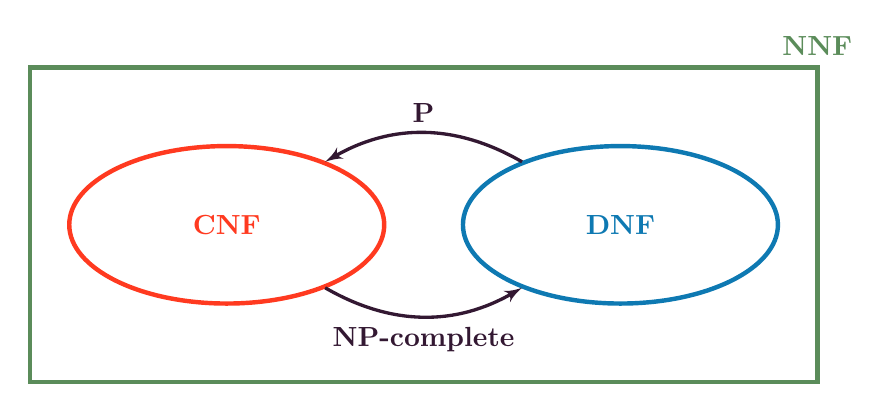
\begin{tikzpicture}
    \draw[ultra thick,palette-orange] (-2.5, 0) ellipse (2cm and 1cm) node (cnf) {\textbf{CNF}};
    \draw[ultra thick,palette-blue] (2.5, 0) ellipse (2cm and 1cm) node (dnf) {\textbf{DNF}};
    \draw[ultra thick,palette-green] (-5, -2.0) rectangle (5, 2.0) node[above] {\textbf{NNF}};
    \pause
    \draw[palette-purple] ($(dnf) + (-1.25, 0.8)$) edge[very thick,bend right=30,->,>=latex']
      node[pos=0.5,above] {\textbf{P}} ($(cnf) + (1.25, 0.8)$);
    \pause
    \draw[palette-purple] ($(cnf) + (1.25, -0.8)$) edge[very thick,bend right=30,->,>=latex']
      node[pos=0.5,below] {\textbf{NP-complete}} ($(dnf) + (-1.25, -0.8)$);
  \end{tikzpicture}
\end{center}

\end{frame}

%%%%%%%%%%%%%%%%%%%%%%%%%%%%%%%%%%%%%%%%%%%%%%%%%%%%%%%%%%%%%%%%%%%%%%%%%%%%%%%%%%%%%%%%%%%%%%%%%%%

\circuitslide{2}

%%%%%%%%%%%%%%%%%%%%%%%%%%%%%%%%%%%%%%%%%%%%%%%%%%%%%%%%%%%%%%%%%%%%%%%%%%%%%%%%%%%%%%%%%%%%%%%%%%%

\setbeamercolor{frametitle}{bg=palette-purple,fg=white}
\begin{frame}{\textbf{Normal Forms in Logic Circuits}}

\vspace{0.5cm}

\begin{minipage}[t][0.7\textheight][t]{0.333\textwidth}
  \textcolor{palette-orange}{\textbf{CNF}}

  \vspace{0.2cm}

  Conjunctive Normal Form

  \vspace{-0.5cm}

  \begin{flalign*}
    &(\textcolor{palette3}{X_1}\textcolor{palette2}{\vee}\textcolor{palette4}{\neg X_2})
    \textcolor{palette1}{\wedge}(\textcolor{palette5}{\neg X_3}\textcolor{palette6}{\vee}
    \textcolor{palette7}{X_4})&
  \end{flalign*}

  \hspace{0.25cm}
  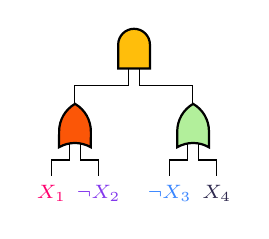
\begin{tikzpicture}
    \newAndNode[fill=palette1]{r}{0, 0};
    \newOrNode[fill=palette2]{d1}{$(r) + (-0.75, -1.0)$};
    \newOrNode[fill=palette6]{d2}{$(r) + (0.75, -1.0)$};
    \draw (r.input 1) -- ++ (0, -0.2) -| (d1);
    \draw (r.input 2) -- ++ (0, -0.2) -| (d2);
    \draw (d1.input 1) -- ++(0, -0.2) -| ($(d1) + (-0.3, -0.6)$) node[below]
      {\scriptsize\textcolor{palette3}{$X_1$}};
    \draw (d1.input 2) -- ++(0, -0.2) -| ($(d1) + (0.3, -0.6)$) node[below]
      {\scriptsize\textcolor{palette4}{$\neg X_2$}};
    \draw (d2.input 1) -- ++(0, -0.2) -| ($(d2) + (-0.3, -0.6)$) node[below]
      {\scriptsize\textcolor{palette5}{$\neg X_3$}};
    \draw (d2.input 2) -- ++(0, -0.2) -| ($(d2) + (0.3, -0.6)$) node[below]
      {\scriptsize\textcolor{palette7}{$X_4$}};
  \end{tikzpicture}
  \pause%
\end{minipage}%
\begin{minipage}[t][0.7\textheight][t]{0.333\textwidth}
  \textcolor{palette-blue}{\textbf{DNF}}

  \vspace{0.2cm}

  Disjunctive Normal Form

  \vspace{-0.5cm}

  \begin{flalign*}
    &(\textcolor{palette3}{\neg Y_1}\textcolor{palette2}{\wedge}\textcolor{palette4}{\neg Y_2})
    \textcolor{palette1}{\vee}(\textcolor{palette5}{Y_3}\textcolor{palette6}{\wedge}
    \textcolor{palette7}{Y_4})&
  \end{flalign*}

  \hspace{0.25cm}
  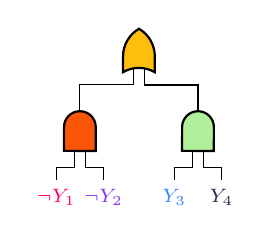
\begin{tikzpicture}
    \newOrNode[fill=palette1]{r}{0, 0};
    \newAndNode[fill=palette2]{d1}{$(r) + (-0.75, -1.0)$};
    \newAndNode[fill=palette6]{d2}{$(r) + (0.75, -1.0)$};
    \draw (r.input 1) -- ++ (0, -0.2) -| (d1);
    \draw (r.input 2) -- ++ (0, -0.2) -| (d2);
    \draw (d1.input 1) -- ++(0, -0.2) -| ($(d1) + (-0.3, -0.6)$) node[below]
      {\scriptsize\textcolor{palette3}{$\neg Y_1$}};
    \draw (d1.input 2) -- ++(0, -0.2) -| ($(d1) + (0.3, -0.6)$) node[below]
      {\scriptsize\textcolor{palette4}{$\neg Y_2$}};
    \draw (d2.input 1) -- ++(0, -0.2) -| ($(d2) + (-0.3, -0.6)$) node[below]
      {\scriptsize\textcolor{palette5}{$Y_3$}};
    \draw (d2.input 2) -- ++(0, -0.2) -| ($(d2) + (0.3, -0.6)$) node[below]
      {\scriptsize\textcolor{palette7}{$Y_4$}};
  \end{tikzpicture}
  \pause%
\end{minipage}%
\begin{minipage}[t][0.7\textheight][t]{0.333\textwidth}
  \textcolor{palette-green}{\textbf{NNF}}

  \vspace{0.2cm}

  Negation Normal Form

  \vspace{-0.5cm}

  \begin{flalign*}
    &\textcolor{palette4}{\neg Z_1}\textcolor{palette1}{\wedge}(\textcolor{palette5}{Z_2}
    \textcolor{palette2}{\vee}\textcolor{palette3}{\neg Z_3})\textcolor{palette6}{\vee}
    \textcolor{palette7}{Z_4}&
  \end{flalign*}

  \hspace{0.25cm}
  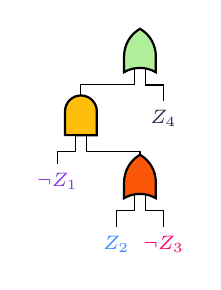
\begin{tikzpicture}
    \newOrNode[fill=palette6]{r}{0, 0};
    \newAndNode[fill=palette1]{d1}{$(r) + (-0.75, -0.8)$};
    \newOrNode[fill=palette2]{d2}{$(d1) + (0.75, -0.8)$};
    \draw (d1.input 1) -- ++(0, -0.2) -| ($(d1) + (-0.3, -0.6)$) node[below]
      {\scriptsize\textcolor{palette4}{$\neg Z_1$}};
    \draw (d1.input 2) -- ++(0, -0.2) -| (d2.output);
    \draw (d2.input 1) -- ++(0, -0.2) -| ($(d2) + (-0.3, -0.6)$) node[below]
      {\scriptsize\textcolor{palette5}{$Z_2$}};
    \draw (d2.input 2) -- ++(0, -0.2) -| ($(d2) + (0.3, -0.6)$) node[below]
      {\scriptsize\textcolor{palette3}{$\neg Z_3$}};
    \draw (r.input 1) -- ++(0, -0.2) -| (d1);
    \draw (r.input 2) -- ++(0, -0.2) -| ($(r) + (0.3, -0.6)$) node[below]
      {\scriptsize\textcolor{palette7}{$Z_4$}};
  \end{tikzpicture}
\end{minipage}

\end{frame}

%%%%%%%%%%%%%%%%%%%%%%%%%%%%%%%%%%%%%%%%%%%%%%%%%%%%%%%%%%%%%%%%%%%%%%%%%%%%%%%%%%%%%%%%%%%%%%%%%%%

\setbeamercolor{frametitle}{bg=palette-purple,fg=white}
\begin{frame}[fragile]{\textbf{Satisfiability and Model Counting in Logic Circuits}}

\newcommand{\scv}[2]{
  \ifnum#1=1\relax
    \textcolor{palette-orange}{#2}
  \else
    \ifnum#1=2\relax
      \textcolor{palette-blue}{#2}
    \else
      \textcolor{palette-green}{#2}
    \fi
  \fi
}

\begin{equation*}
  \phi(\scv{1}{X}, \scv{2}{\scv{2}{Y}}, \scv{3}{\scv{3}{Z}}) = [\scv{1}{X} \wedge (\neg \scv{2}{Y} \vee \scv{3}{Z})] \vee [(\neg \scv{3}{Z} \vee \scv{2}{Y}) \wedge\neg \scv{1}{X}]
\end{equation*}\pause%
\vspace{-0.5cm}

\only<2-4>{
\begin{equation*}
  \text{Are there }\scv{1}{X} = \scv{1}{x},\,\scv{2}{Y} = \scv{2}{y},\,\scv{3}{Z} = \scv{3}{z}
  \text{ s.t. } \phi(\scv{1}{X}=\scv{1}{x}, \scv{2}{Y}=\scv{2}{y}, \scv{3}{Z}=\scv{3}{z}) = 1?
\end{equation*}\pause%
}%
\only<5->{
\begin{equation*}
  \text{How \textit{many} }\scv{1}{X} = \scv{1}{x},\,\scv{2}{Y} = \scv{2}{y},\,
  \scv{3}{Z} = \scv{3}{z} \text{ s.t. } \phi(\scv{1}{X}=\scv{1}{x},\scv{2}{Y}=\scv{2}{y},\scv{3}{Z}=\scv{3}{z}) = 1?
\end{equation*}\pause%
}

\vspace{-0.5cm}

\onslide<3,4,5,6>{
\begin{center}
  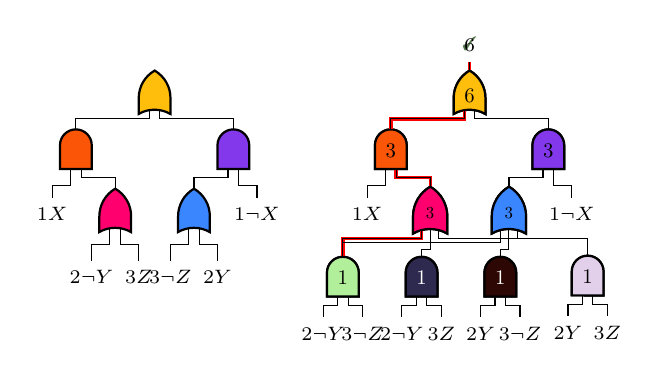
\begin{tikzpicture}
    \newOrNode[fill=palette1]{n}{-2, 0};
    \newAndNode[fill=palette2]{l}{$(n) + (-1, -0.7)$};
    \draw (n.input 1) -- ++(0, -0.1) -| (l.output);
    \draw (l.input 1) -- ++(0, -0.2) -| ($(l) + (-0.3, -0.6)$) node[below]
      {\scriptsize$\scv{1}{X}$};
    \newOrNode[fill=palette3]{lr}{$(l) + (0.5, -0.8)$};
    \draw (l.input 2) -- ++(0, -0.1) -| (lr.output);
    \draw (lr.input 1) -- ++(0, -0.2) -| ($(lr) + (-0.3, -0.6)$) node[below]
      {\scriptsize$\scv{2}{\neg Y}$};
    \draw (lr.input 2) -- ++(0, -0.2) -| ($(lr) + (0.3, -0.6)$) node[below]
      {\scriptsize$\scv{3}{Z}$};
    \newAndNode[fill=palette4]{r}{$(n) + (1, -0.7)$};
    \draw (n.input 2) -- ++(0, -0.1) -| (r.output);
    \draw (r.input 2) -- ++(0, -0.2) -| ($(r) + (0.3, -0.6)$) node[below]
      {\scriptsize$\scv{1}{\neg X}$};
    \newOrNode[fill=palette5]{rl}{$(r) + (-0.5, -0.8)$};
    \draw (r.input 1) -- ++(0, -0.1) -| (rl.output);
    \draw (rl.input 1) -- ++(0, -0.2) -| ($(rl) + (-0.3, -0.6)$) node[below]
      {\scriptsize$\scv{3}{\neg Z}$};
    \draw (rl.input 2) -- ++(0, -0.2) -| ($(rl) + (0.3, -0.6)$) node[below]
      {\scriptsize$\scv{2}{Y}$};

    \onslide<4,6>{
    \onslide<4>{\newOrNode[fill=palette1]{n}{2, 0};}
    \onslide<6>{\newNamedOrNode[fill=palette1]{n}{2, 0}{6};}
    \onslide<4>{\newAndNode[fill=palette2]{l}{$(n) + (-1, -0.7)$};}
    \onslide<6>{\newNamedAndNode[fill=palette2]{l}{$(n) + (-1, -0.7)$}{3};}
    \onslide<4>{\draw[red,very thick] (n.input 1) -- ++(0, -0.1) -| (l.output);}
    \onslide<6>{\draw (n.input 1) -- ++(0, -0.1) -| (l.output);}
    \draw (l.input 1) -- ++(0, -0.2) -| ($(l) + (-0.3, -0.6)$) node[below]
      {\scriptsize$\scv{1}{X}$};
    \onslide<4>{\newOrNode[fill=palette3,inputs=nnn,scale=0.9]{lr}{$(l) + (0.5, -0.8)$};}
    \onslide<6>{\newNamedOrNode[fill=palette3,inputs=nnn,scale=0.9]{lr}{$(l) + (0.5, -0.8)$}{3};}
    \onslide<4>{\draw[red,very thick] (l.input 2) -- ++(0, -0.1) -| (lr.output);}
    \onslide<6>{\draw (l.input 2) -- ++(0, -0.1) -| (lr.output);}
    \onslide<4>{\newAndNode[fill=palette4]{r}{$(n) + (1, -0.7)$};}
    \onslide<6>{\newNamedAndNode[fill=palette4]{r}{$(n) + (1, -0.7)$}{3};}
    \draw (n.input 2) -- ++(0, -0.1) -| (r.output);
    \newOrNode[fill=palette5,inputs=nnn,scale=0.9]{rl}{$(r) + (-0.5, -0.8)$};
    \onslide<6>{\newNamedOrNode[fill=palette5,inputs=nnn,scale=0.9]{rl}{$(r) + (-0.5, -0.8)$}{3};}
    \draw (r.input 1) -- ++(0, -0.1) -| (rl.output);
    \draw (r.input 2) -- ++(0, -0.2) -| ($(r) + (0.3, -0.6)$) node[below]
      {\scriptsize$\scv{1}{\neg X}$};

    \newAndNode[fill=palette6]{b1}{$(lr.input 1) + (-1.0, -0.6)$};
    \draw (b1.input 1) -- ++(0, -0.1) -| ($(b1) + (-0.25, -0.5)$) node[below]
      {\scriptsize$\scv{2}{\neg Y}$};
    \draw (b1.input 2) -- ++(0, -0.1) -| ($(b1) + (0.25, -0.5)$) node[below]
      {\scriptsize$\scv{3}{\neg Z}$};
    \newAndNode[fill=palette7]{b2}{$(lr.input 1) + (0.0, -0.6)$};
    \draw (b2.input 1) -- ++(0, -0.1) -| ($(b2) + (-0.25, -0.5)$) node[below]
      {\scriptsize$\scv{2}{\neg Y}$};
    \draw (b2.input 2) -- ++(0, -0.1) -| ($(b2) + (0.25, -0.5)$) node[below]
      {\scriptsize$\scv{3}{Z}$};
    \newAndNode[fill=palette8]{b3}{$(rl.input 1) + (0.0, -0.6)$};
    \draw (b3.input 1) -- ++(0, -0.1) -| ($(b3) + (-0.25, -0.5)$) node[below]
      {\scriptsize$\scv{2}{Y}$};
    \draw (b3.input 2) -- ++(0, -0.1) -| ($(b3) + (0.25, -0.5)$) node[below]
      {\scriptsize$\scv{3}{\neg Z}$};
    \newAndNode[fill=palette9]{b4}{$(rl.input 2) + (1.0, -0.6)$};
    \draw (b4.input 1) -- ++(0, -0.1) -| ($(b4) + (-0.25, -0.5)$) node[below]
      {\scriptsize$\scv{2}{Y}$};
    \draw (b4.input 2) -- ++(0, -0.1) -| ($(b4) + (0.25, -0.5)$) node[below]
      {\scriptsize$\scv{3}{Z}$};

    \onslide<6>{\newNamedAndNode[fill=palette6]{b1}{$(lr.input 1) + (-1.0, -0.6)$}{1};}
    \onslide<6>{\newNamedAndNode[fill=palette7]{b2}{$(lr.input 1) + (0.0, -0.6)$}{\color{white}1};}
    \onslide<6>{\newNamedAndNode[fill=palette8]{b3}{$(rl.input 1) + (0.0, -0.6)$}{\color{white}1};}
    \onslide<6>{\newNamedAndNode[fill=palette9]{b4}{$(rl.input 2) + (1.0, -0.6)$}{1};}

    \onslide<4>{\draw[red,very thick] (lr.input 1) -- ++(0, -0.1) -| (b1.output);}
    \onslide<6>{\draw (lr.input 1) -- ++(0, -0.1) -| (b1.output);}
    \draw (lr.input 2) -- ++(0, -0.25) -| (b2.output);
    \draw (lr.input 3) -- ++(0, -0.1) -| (b4.output);

    \draw (rl.input 1) -- ++(0, -0.15) -| (b1.output);
    \draw (rl.input 2) -- ++(0, -0.25) -| (b3.output);
    \draw (rl.input 3) -- ++(0, -0.1) -| (b4.output);

    \onslide<4>{
      \draw[red,very thick] (n.output) -- ($(n.output) + (0, 0.1)$) node[above] {\scriptsize\cmark};
    }
    \onslide<6>{\draw (n.output) -- ($(n.output) + (0, 0.1)$) node[above] {\scriptsize 6};}
    }
  \end{tikzpicture}
\end{center}
}

\only<1-3,5>{
  \begin{center}
    \phantom{\textbf{A}}
  \end{center}
}\only<4>{
\begin{center}
  $\mathbf{SAT}=\text{\cmark}$
\end{center}
}\only<6>{
\begin{center}
  $\mathbf{\#SAT}=6$
\end{center}
}

\end{frame}

%%%%%%%%%%%%%%%%%%%%%%%%%%%%%%%%%%%%%%%%%%%%%%%%%%%%%%%%%%%%%%%%%%%%%%%%%%%%%%%%%%%%%%%%%%%%%%%%%%%
\circuitslide{3}
%%%%%%%%%%%%%%%%%%%%%%%%%%%%%%%%%%%%%%%%%%%%%%%%%%%%%%%%%%%%%%%%%%%%%%%%%%%%%%%%%%%%%%%%%%%%%%%%%%%

\setbeamercolor{frametitle}{bg=palette-purple,fg=white}
\begin{frame}[fragile]{\textbf{The World of Logic Circuits}}

\begin{center}
\resizebox{!}{0.75\textheight}{
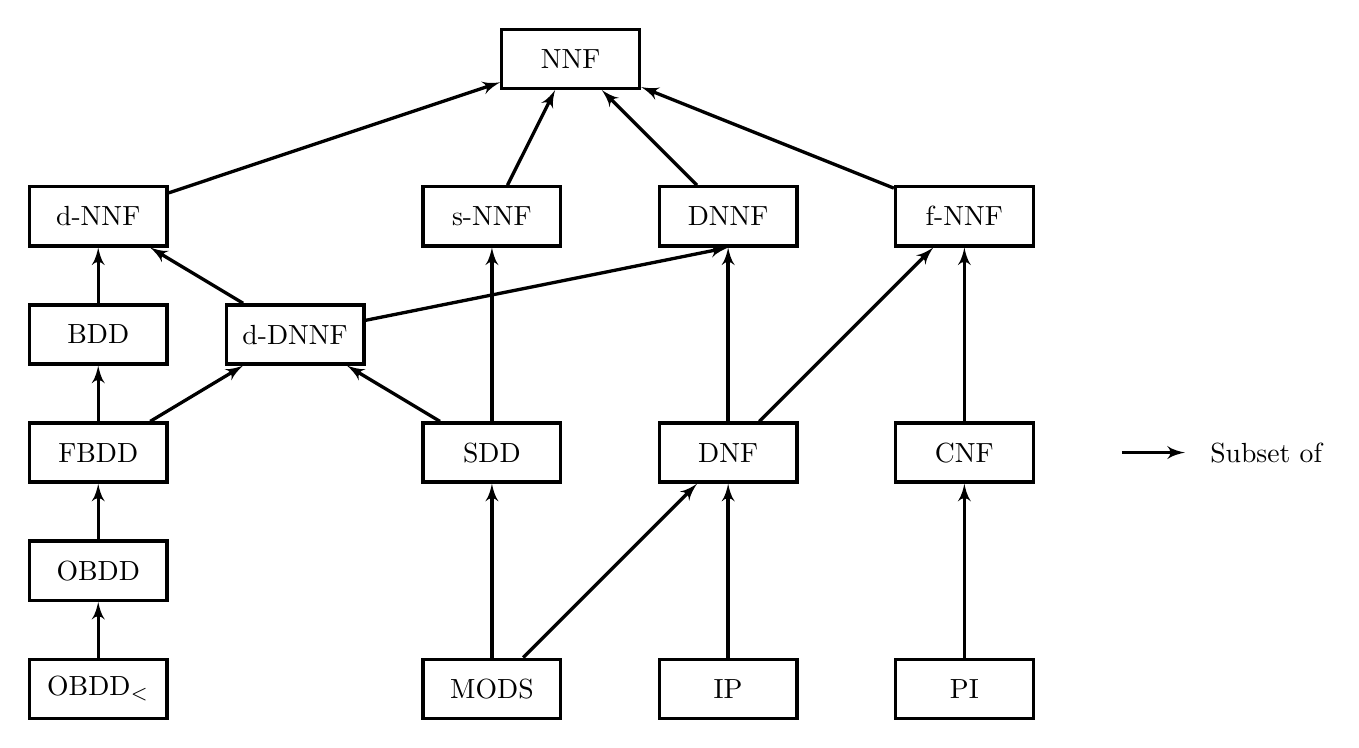
\begin{tikzpicture}[lang/.style={very thick,rectangle,draw,minimum width=1.75cm,minimum
  height=0.75cm},ledge/.style={->,>=latex',very thick}]
  \node[lang] (nnf) at (0, 0) {NNF};

  \node[lang] (d-nnf) at ($(nnf) + (-6, -2.0)$) {d-NNF};
  \node[lang] (bdd) at ($(d-nnf) + (0, -1.5)$) {BDD};
  \node[lang] (fbdd) at ($(bdd) + (0, -1.5)$) {FBDD};
  \node[lang] (obdd) at ($(fbdd) + (0, -1.5)$) {OBDD};
  \node[lang] (obddlt) at ($(obdd) + (0, -1.5)$) {OBDD$_<$};
  \node[lang] (d-dnnf) at ($(bdd) + (2.5, 0)$) {d-DNNF};

  \node[lang] (s-nnf) at ($(nnf) + (-1, -2.0)$) {s-NNF};
  \node[lang] (sdd) at ($(s-nnf) + (0, -3.0)$) {SDD};
  \node[lang] (mods) at (obddlt -| sdd) {MODS};

  \node[lang] (dnnf) at ($(nnf) + (2, -2.0)$) {DNNF};
  \node[lang] (dnf) at ($(dnnf) + (0, -3.0)$) {DNF};
  \node[lang] (ip) at (obddlt -| dnf) {IP};

  \node[lang] (f-nnf) at ($(nnf) + (5, -2.0)$) {f-NNF};
  \node[lang] (cnf) at ($(f-nnf) + (0, -3.0)$) {CNF};
  \node[lang] (pi) at (obddlt -| cnf) {PI};

  \draw[ledge] (obddlt) -- (obdd); \draw[ledge] (obdd) -- (fbdd);
  \draw[ledge] (fbdd) -- (bdd); \draw[ledge] (bdd) -- (d-nnf);
  \draw[ledge] (d-nnf) -- (nnf); \draw[ledge] (fbdd) -- (d-dnnf);
  \draw[ledge] (d-dnnf) -- (d-nnf); \draw[ledge] (d-dnnf) -- (dnnf.south);
  \draw[ledge] (mods) -- (sdd); \draw[ledge] (sdd) -- (s-nnf);
  \draw[ledge] (sdd) -- (d-dnnf); \draw[ledge] (s-nnf) -- (nnf);
  \draw[ledge] (ip) -- (dnf); \draw[ledge] (dnf) -- (dnnf);
  \draw[ledge] (dnnf) -- (nnf); \draw[ledge] (dnf) -- (f-nnf);
  \draw[ledge] (pi) -- (cnf); \draw[ledge] (cnf) -- (f-nnf);
  \draw[ledge] (f-nnf) -- (nnf); \draw[ledge] (mods) -- (dnf);

  \node[anchor=west] (leg) at ($(cnf) + (3, 0)$) {Subset of};
  \draw[ledge] ($(leg.west) + (-1, 0)$) -- ($(leg.west) + (-0.2, 0)$);
\end{tikzpicture}
}
\end{center}

\textcolor{dark gray}{\scriptsize\citep{darwiche02}}

\end{frame}

%%%%%%%%%%%%%%%%%%%%%%%%%%%%%%%%%%%%%%%%%%%%%%%%%%%%%%%%%%%%%%%%%%%%%%%%%%%%%%%%%%%%%%%%%%%%%%%%%%%

\setbeamercolor{frametitle}{bg=palette-purple,fg=white}
\begin{frame}[fragile]{\textbf{Succinctness in Logic Circuits}}

\begin{center}
\resizebox{!}{0.75\textheight}{
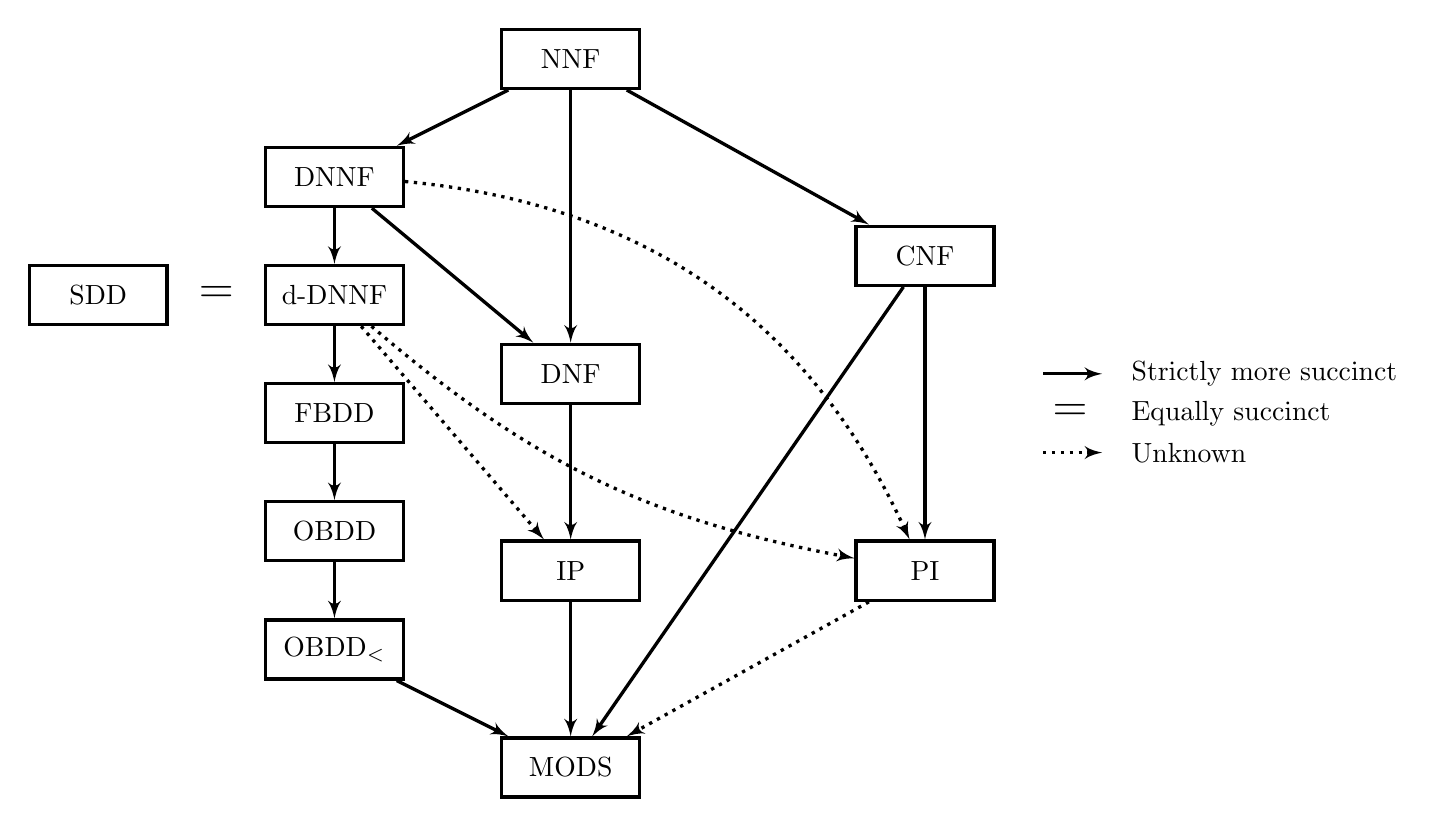
\begin{tikzpicture}[lang/.style={very thick,rectangle,draw,minimum width=1.75cm,minimum
  height=0.75cm},ledge/.style={->,>=latex',very thick}]
  \node[lang] (nnf) at (0, 0) {NNF};
  \node[lang] (dnnf) at ($(nnf) + (-3, -1.5)$) {DNNF};
  \node[lang] (d-dnnf) at ($(dnnf) + (0, -1.5)$) {d-DNNF};
  \node[lang] (sd-dnnf) at ($(d-dnnf) + (-3, 0)$) {SDD};
  \node[lang] (fbdd) at ($(d-dnnf) + (0, -1.5)$) {FBDD};
  \node[lang] (obdd) at ($(fbdd) + (0, -1.5)$) {OBDD};
  \node[lang] (obddlt) at ($(obdd) + (0, -1.5)$) {OBDD$_<$};
  \node[lang] (dnf) at ($(nnf) + (0, -4.0)$) {DNF};
  \node[lang] (ip) at ($(dnf) + (0, -2.5)$) {IP};
  \node[lang] (mods) at ($(ip) + (0, -2.5)$) {MODS};
  \node[lang] (cnf) at ($(nnf) + (4.5, -2.5)$) {CNF};
  \node[lang] (pi) at ($(cnf) + (0, -4)$) {PI};

  \path (d-dnnf) -- (sd-dnnf) node[midway] {\LARGE =};
  \draw[ledge] (nnf) -- (dnnf);
  \draw[ledge] (dnnf) -- (d-dnnf);
  \draw[ledge] (d-dnnf) -- (fbdd);
  \draw[ledge] (fbdd) -- (obdd);
  \draw[ledge] (obdd) -- (obddlt);
  \draw[ledge] (obddlt) -- (mods);
  \draw[ledge] (dnnf) -- (dnf);
  \draw[ledge] (dnf) -- (ip);
  \draw[ledge] (ip) -- (mods);
  \draw[ledge] (nnf) -- (cnf);
  \draw[ledge] (cnf) -- (pi);
  \draw[ledge] (cnf) -- (mods);
  \draw[ledge] (nnf) -- (dnf);
  \draw[ledge,dotted] (pi) -- (mods);
  \draw[ledge,dotted] (dnnf) to[bend left] (pi);
  \draw[ledge,dotted] (d-dnnf) to[bend right=15] (pi);
  \draw[ledge,dotted] (d-dnnf) -- (ip);

  \node[anchor=west] (leg-succ) at ($(cnf) + (2.5, -1.5)$) {Strictly more succinct};
  \node[anchor=west] (leg-eqsucc) at ($(leg-succ.west) + (0, -0.5)$) {Equally succinct};
  \node[anchor=west] (leg-unk) at ($(leg-eqsucc.west) + (0, -0.5)$) {Unknown};
  \draw[ledge] ($(leg-succ.west) + (-1.0, 0)$) -- ($(leg-succ.west) + (-0.25, 0)$);
  \node[anchor=west] at ($(leg-eqsucc.west) + (-1.0, 0)$) {\LARGE =};
  \draw[ledge,dotted] ($(leg-unk.west) + (-1.0, 0)$) -- ($(leg-unk.west) + (-0.25, 0)$);
\end{tikzpicture}
}
\end{center}

\textcolor{dark gray}{\scriptsize\citep{darwiche02}}

\end{frame}

%%%%%%%%%%%%%%%%%%%%%%%%%%%%%%%%%%%%%%%%%%%%%%%%%%%%%%%%%%%%%%%%%%%%%%%%%%%%%%%%%%%%%%%%%%%%%%%%%%%

\setbeamercolor{frametitle}{bg=palette-purple,fg=white}
\begin{frame}[fragile]{\textbf{Querying in Logic Circuits}}

\begin{center}
  \scriptsize
  \begin{minipage}{0.6\textwidth}
    \begin{tabular}{l|cccccccc}
      \textbf{L} & \textbf{CO} & \textbf{VA} & \textbf{CE} & \textbf{IM} & \textbf{EQ} & \textbf{SE}
                 & \textbf{CT} & \textbf{ME}\\
      \hline
          NNF & \omark & \omark & \omark & \omark & \omark & \omark & \omark & \omark\\
         DNNF & \cmark & \omark & \cmark & \omark & \omark & \omark & \omark & \cmark\\
        d-NNF & \omark & \omark & \omark & \omark & \omark & \omark & \omark & \omark\\
        s-NNF & \omark & \omark & \omark & \omark & \omark & \omark & \omark & \omark\\
        f-NNF & \omark & \omark & \omark & \omark & \omark & \omark & \omark & \omark\\
       d-DNNF & \cmark & \cmark & \cmark & \cmark &    ?   & \omark & \cmark & \cmark\\
          SDD & \cmark & \cmark & \cmark & \cmark &    ?   & \omark & \cmark & \cmark\\
          BDD & \omark & \omark & \omark & \omark & \omark & \omark & \omark & \omark\\
         FBDD & \cmark & \cmark & \cmark & \cmark &    ?   & \omark & \cmark & \cmark\\
         OBDD & \cmark & \cmark & \cmark & \cmark & \cmark & \omark & \cmark & \cmark\\
      OBDD$_<$& \cmark & \cmark & \cmark & \cmark & \cmark & \cmark & \cmark & \cmark\\
          DNF & \cmark & \omark & \cmark & \omark & \omark & \omark & \omark & \cmark\\
          CNF & \omark & \cmark & \omark & \cmark & \omark & \omark & \omark & \omark\\
           PI & \cmark & \cmark & \cmark & \cmark & \cmark & \cmark & \omark & \cmark\\
           IP & \cmark & \cmark & \cmark & \cmark & \cmark & \cmark & \omark & \cmark\\
         MODS & \cmark & \cmark & \cmark & \cmark & \cmark & \cmark & \cmark & \cmark\\
    \end{tabular}
  \end{minipage}%
  \begin{minipage}{0.4\textwidth}
    \begin{tabular}{l|l}
      \textbf{Notation} & \textbf{Query}\\
      \hline
      \textbf{CO} & Consistency check\\
      \textbf{VA} & Validity check\\
      \textbf{CE} & Clausal entailment check\\
      \textbf{IM} & Implicant check\\
      \textbf{EQ} & Equivalence check\\
      \textbf{SE} & Sentential entailment check\\
      \textbf{CT} & Model counting\\
      \textbf{ME} & Model enumeration\\
    \end{tabular}

    \vspace{0.5cm}

    \begin{tabular}{l|l}
      \textbf{Notation} & \textbf{Description}\\
      \hline
      \cmark & In P\\
      \xmark & Not in P\\
      \omark & Not in P unless $\textup{P}=\textup{NP}$\\
      ? & Unknown\\
    \end{tabular}
  \end{minipage}
\end{center}

\vfill
\textcolor{dark gray}{\scriptsize\citep{darwiche02}}

\end{frame}

%%%%%%%%%%%%%%%%%%%%%%%%%%%%%%%%%%%%%%%%%%%%%%%%%%%%%%%%%%%%%%%%%%%%%%%%%%%%%%%%%%%%%%%%%%%%%%%%%%%

\setbeamercolor{frametitle}{bg=palette-purple,fg=white}
\begin{frame}[fragile]{\textbf{Transformations in Logic Circuits}}

\begin{center}
  \scriptsize
  \begin{minipage}{0.65\textwidth}
    \begin{tabular}{l|cccccccc}
      \textbf{L} & \textbf{CD} & \textbf{FO} & \textbf{SFO} & \textbf{$\wedge$C} &
      \textbf{$\wedge$BC} & \textbf{$\vee$C} & \textbf{$\vee$BC} & \textbf{$\neg$C}\\
      \hline
          NNF & \cmark & \omark & \cmark & \cmark & \cmark & \cmark & \cmark & \cmark\\
         DNNF & \cmark & \cmark & \cmark & \omark & \omark & \cmark & \cmark & \omark\\
        d-NNF & \cmark & \omark & \cmark & \cmark & \cmark & \cmark & \cmark & \cmark\\
        s-NNF & \cmark & \omark & \cmark & \cmark & \cmark & \cmark & \cmark & \cmark\\
        f-NNF & \cmark & \omark & \cmark & \xmark & \xmark & \xmark & \xmark & \cmark\\
       d-DNNF & \cmark & \omark & \omark & \omark & \omark & \omark & \omark & \cmark\\
          SDD & \cmark & \omark & \omark & \omark & \omark & \omark & \omark & \cmark\\
          BDD & \cmark & \omark & \cmark & \cmark & \cmark & \cmark & \cmark & \cmark\\
         FBDD & \cmark & \xmark & \omark & \xmark & \omark & \xmark & \omark & \cmark\\
         OBDD & \cmark & \xmark & \cmark & \xmark & \omark & \xmark & \omark & \cmark\\
      OBDD$_<$& \cmark & \xmark & \cmark & \xmark & \cmark & \xmark & \cmark & \cmark\\
          DNF & \cmark & \cmark & \cmark & \xmark & \cmark & \cmark & \cmark & \xmark\\
          CNF & \cmark & \omark & \cmark & \cmark & \cmark & \xmark & \cmark & \xmark\\
           PI & \cmark & \cmark & \cmark & \xmark & \xmark & \xmark & \cmark & \xmark\\
           IP & \cmark & \xmark & \xmark & \xmark & \cmark & \xmark & \xmark & \xmark\\
         MODS & \cmark & \cmark & \cmark & \xmark & \cmark & \xmark & \xmark & \xmark\\
    \end{tabular}
  \end{minipage}%
  \begin{minipage}{0.35\textwidth}
    \begin{tabular}{l|l}
      \textbf{Notation} & \textbf{Query}\\
      \hline
      \textbf{CD} & Conditioning\\
      \textbf{FO} & Forgetting\\
      \textbf{SFO} & Singleton forgetting\\
      \textbf{$\wedge$C} & Conjunction\\
      \textbf{$\wedge$BC} & Bounded conjunction\\
      \textbf{$\vee$C} & Disjunction\\
      \textbf{$\vee$BC} & Bounded disjunction\\
      \textbf{$\neg$C} & Negation\\
    \end{tabular}

    \vspace{0.5cm}

    \begin{tabular}{l|l}
      \textbf{Notation} & \textbf{Description}\\
      \hline
      \cmark & In P\\
      \xmark & Not in P\\
      \omark & Not in P unless $\textup{P}=\textup{NP}$\\
      ? & Unknown\\
    \end{tabular}
  \end{minipage}
\end{center}

\vfill
\textcolor{dark gray}{\scriptsize\citep{darwiche02}}

\end{frame}

%%%%%%%%%%%%%%%%%%%%%%%%%%%%%%%%%%%%%%%%%%%%%%%%%%%%%%%%%%%%%%%%%%%%%%%%%%%%%%%%%%%%%%%%%%%%%%%%%%%

\circuitslide{4}

%%%%%%%%%%%%%%%%%%%%%%%%%%%%%%%%%%%%%%%%%%%%%%%%%%%%%%%%%%%%%%%%%%%%%%%%%%%%%%%%%%%%%%%%%%%%%%%%%%%

% If is final version
\def\isfinalversion{1}
\ifx\isfinalversion\undefined
  \newcommand{\nsamples}{10}
\else
  \newcommand{\nsamples}{50}
\fi
\newenvironment{vhcenterb}{\vspace*{\fill}\begin{center}}{\end{center}\vspace*{\fill}}

\setbeamercolor{frametitle}{bg=palette-purple,fg=white}
\begin{frame}[fragile]{\textbf{Probabilistic Circuits}}

\vspace{-0.5cm}

\begin{center}
\newcommand\xmone{2}%
\newcommand\xsone{0.5}%
\newcommand\xmtwo{4}%
\newcommand\xstwo{0.8}%
\newcommand\ymone{3}%
\newcommand\ysone{0.7}%
\newcommand\ymtwo{5}%
\newcommand\ystwo{0.4}%
\begin{minipage}[t][0.75\textheight][t]{0.45\textwidth}
\begin{vhcenterb}
  \resizebox{\textwidth}{!}{
  \begin{tikzpicture}
    \pgfplotsset{
      every axis/.append style={
        axis line style={->,>=latex'},
        tick label style={font={\scriptsize\bfseries}},
        x tick label style={color=white,below},
        y tick label style={color=white,left},
        grid style={black,dashed},
      }
    }
    \begin{axis}[
      no markers, domain=0:7, samples=\nsamples,
      width=5cm, height=3.5cm,
      xtick={2}, ytick={0.25},
      xticklabels={\colorbox{boxblue}{\textbf{2}}},
      yticklabels={\colorbox{boxred}{\textbf{0.25}}},
      axis lines*=left, xlabel=$x$, ylabel=$p(x)$,
      every axis y label/.style={font=\scriptsize,at={(axis description cs:-0.1,0.9)},anchor=south},
      every axis x label/.style={font=\scriptsize,at=(current axis.right of origin),anchor=west},
      enlargelimits=false, clip=false, axis on top,
      grid = major
    ]
      \path[name path=axis] (axis cs:0,0) -- (axis cs:7,0);
      \addplot[very thick,boxteal,name path=g1] {gauss(\xmone,\xsone)};
      \addplot[very thick,boxorange,name path=g2] {gauss(\xmtwo,\xstwo)};
      \addplot[very thick,boxred] {mixgauss2(\xmone,\xsone,\xmtwo,\xstwo,0.3,0.7)};
      \addplot[boxteal!60] fill between [of=g1 and axis];
      \addplot[boxorange!50] fill between [of=g2 and axis];
      \node at (axis cs:\xmone,{egauss(\xmone,\xsone,\xmone)+0.1}) {\tiny$\mu_1=\xmone$};
      \node at (axis cs:\xmtwo,{egauss(\xmtwo,\xstwo,\xmtwo)+0.1}) {\tiny$\mu_2=\xmtwo$};
    \end{axis}
  \end{tikzpicture}
  \begin{tikzpicture}
    \pgfplotsset{
      every axis/.append style={
        axis line style={->,>=latex'},
        tick label style={font={\scriptsize\bfseries}},
        x tick label style={color=white,below},
        y tick label style={color=white,left},
        grid style={black,dashed},
      }
    }
    \begin{axis}[
      no markers, domain=1:7, samples=\nsamples,
      width=5cm, height=3.5cm,
      xtick={4}, ytick={0.14},
      xticklabels={\colorbox{boxblue}{\textbf{4}}},
      yticklabels={\colorbox{boxpurple}{\textbf{0.14}}},
      axis lines*=left, xlabel=$y$, ylabel=$p(y)$,
      every axis y label/.style={font=\scriptsize,at={(axis description cs:-0.1,0.9)},anchor=south},
      every axis x label/.style={font=\scriptsize,at=(current axis.right of origin),anchor=west},
      enlargelimits=false, clip=false, axis on top,
      grid = major
    ]
      \path[name path=axis] (axis cs:0,0) -- (axis cs:7,0);
      \addplot[very thick,boxpink,name path=g1] {gauss(\ymone,\ysone)};
      \addplot[very thick,boxgoldenrod,name path=g2] {gauss(\ymtwo,\ystwo)};
      \addplot[very thick,boxpurple] {mixgauss2(\ymone,\ysone,\ymtwo,\ystwo,0.6,0.4)};
      \addplot[boxpink!40] fill between [of=g1 and axis];
      \addplot[boxgoldenrod!50] fill between [of=g2 and axis];
      \node at (axis cs:\ymone,{egauss(\ymone,\ysone,\ymone)+0.1}) {\tiny$\mu_3=\ymone$};
      \node at (axis cs:\ymtwo,{egauss(\ymtwo,\ystwo,\ymtwo)+0.1}) {\tiny$\mu_4=\ymtwo$};
    \end{axis}
  \end{tikzpicture}
  }
  \begin{tikzpicture}
    \pgfplotsset{
      every axis/.append style={
        axis line style={->,>=latex'},
        axis lines=center,
        grid style={black,dashed},
        tick label style={font={\scriptsize\bfseries}},
        x tick label style={color=white,below},
        y tick label style={color=white,right},
        z tick label style={color=white,left},
      }
    }
    \begin{axis}[
      no markers, width=0.8\columnwidth,
      xtick={2}, ytick={4}, ztick={0.035},
      xticklabels={\colorbox{boxblue}{\textbf{2}}},
      yticklabels={\colorbox{boxblue}{\textbf{4}}},
      zticklabels={\colorbox{boxgreen}{\textbf{0.035}}},
      xlabel={\scriptsize$x$}, ylabel={\scriptsize$y$}, zlabel={\scriptsize$p(x,y)$},
      axis lines*=left,
      xlabel style={anchor=north west},
      ylabel style={anchor=south west},
      zlabel style={anchor=south east},
      enlargelimits=false, clip=false, axis on top,
      grid = major
    ]
      \addplot3[
        surf, samples=\nsamples,
        domain=0.5:6.5,
        y domain=1:6
      ] {((0.3*exp(-((x-\xmone)^2)/(2*\xsone^2))/\xsone+0.7*exp(-((x-\xmtwo)^2)/(2*\xstwo^2))/\xstwo)/2.5066)*(((0.6*exp(-((y-\ymone)^2)/(2*\ysone^2))/\ysone+0.4*exp(-((y-\ymtwo)^2)/(2*\ystwo^2))/\ystwo)/2.5066))};
    \end{axis}
  \end{tikzpicture}
\end{vhcenterb}
\end{minipage}
\begin{minipage}[t][0.7\textheight][t]{0.45\textwidth}
\begin{vhcenterb}
  \resizebox{0.7\textwidth}{!}{
  \begin{tikzpicture}
    \newProdNode[fill=boxgreen]{r}{0,0};
    \newSumNode[fill=boxred!70]{p}{$(r) + (-1.25,-0.75)$};
    \newSumNode[fill=boxpurple!60]{q}{$(r) + (1.25,-0.75)$};
    \newGaussNode[fill=boxteal]{x1}{$(p) + (-0.6,-1)$};
    \newGaussNode[fill=boxorange!80]{x2}{$(p) + (0.65,-1)$};
    \newGaussNode[fill=boxpink!50]{y1}{$(q) + (-0.6,-1)$};
    \newGaussNode[fill=boxgoldenrod!70]{y2}{$(q) + (0.6,-1)$};
    \draw[edge] (r) edge (p);
    \draw[edge] (r) edge (q);
    \draw[edge] (p) edge (x1);
    \draw[edge] (p) edge (x2);
    \draw[edge] (q) edge (y1);
    \draw[edge] (q) edge (y2);
    \node at ($(p) + (-0.5,-0.4)$) {\scriptsize$.3$};
    \node at ($(p) + (0.5,-0.4)$) {\scriptsize$.7$};
    \node at ($(q) + (-0.5,-0.4)$) {\scriptsize$.6$};
    \node at ($(q) + (0.5,-0.4)$) {\scriptsize$.4$};
    \node (l1) at ($(x1) + (0,-0.5)$) {\scriptsize$\mathcal{N}_1(\xmone,\xsone)$};
    \node (l2) at ($(x2) + (0,-0.5)$) {\scriptsize$\mathcal{N}_2(\xmtwo,\xstwo)$};
    \node (l3) at ($(y1) + (0,-0.5)$) {\scriptsize$\mathcal{N}_3(\ymone,\ysone)$};
    \node (l4) at ($(y2) + (0,-0.5)$) {\scriptsize$\mathcal{N}_4(\ymtwo,\ystwo)$};
  \end{tikzpicture}
  }
  \resizebox{0.7\textwidth}{!}{
  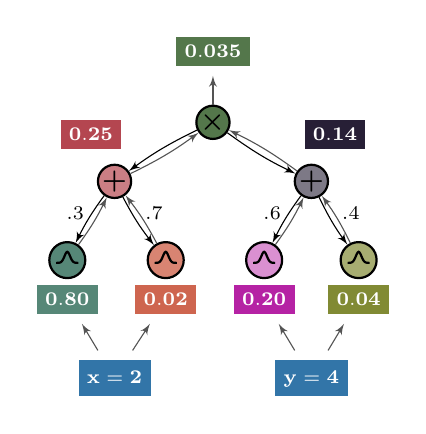
\begin{tikzpicture}
    \newProdNode[fill=boxgreen]{r}{0,0};
    \newSumNode[fill=boxred!70]{p}{$(r) + (-1.25,-0.75)$};
    \newSumNode[fill=boxpurple!60]{q}{$(r) + (1.25,-0.75)$};
    \newGaussNode[fill=boxteal]{x1}{$(p) + (-0.6,-1)$};
    \newGaussNode[fill=boxorange!80]{x2}{$(p) + (0.65,-1)$};
    \newGaussNode[fill=boxpink!50]{y1}{$(q) + (-0.6,-1)$};
    \newGaussNode[fill=boxgoldenrod!70]{y2}{$(q) + (0.6,-1)$};
    \draw[edge] (r) edge[bend right=5] (p);
    \draw[edge] (r) edge[bend right=5] (q);
    \draw[edge] (p) edge[bend right=5] (x1);
    \draw[edge] (p) edge[bend right=5] (x2);
    \draw[edge] (q) edge[bend right=5] (y1);
    \draw[edge] (q) edge[bend right=5] (y2);
    \node at ($(p) + (-0.5,-0.4)$) {\scriptsize$.3$};
    \node at ($(p) + (0.5,-0.4)$) {\scriptsize$.7$};
    \node at ($(q) + (-0.5,-0.4)$) {\scriptsize$.6$};
    \node at ($(q) + (0.5,-0.4)$) {\scriptsize$.4$};
    \node (l1) at ($(x1) + (0,-0.5)$) {\scriptsize\colorbox{boxteal}{\color{white}$\mathbf{0.80}$}};
    \node (l2) at ($(x2) + (0,-0.5)$) {\scriptsize\colorbox{boxorange}{\color{white}$\mathbf{0.02}$}};
    \node (l3) at ($(y1) + (0,-0.5)$) {\scriptsize\colorbox{boxpink}{\color{white}$\mathbf{0.20}$}};
    \node (l4) at ($(y2) + (0,-0.5)$) {\scriptsize\colorbox{boxgoldenrod}{\color{white}$\mathbf{0.04}$}};
    \draw[edge,boxdgray] (p) edge[bend left=-5] (r);
    \draw[edge,boxdgray] (q) edge[bend left=-5] (r);
    \draw[edge,boxdgray] (x1) edge[bend left=-5] (p);
    \draw[edge,boxdgray] (x2) edge[bend left=-5] (p);
    \draw[edge,boxdgray] (y1) edge[bend left=-5] (q);
    \draw[edge,boxdgray] (y2) edge[bend left=-5] (q);
    \node at ($(p) + (-0.3,0.6)$) {\scriptsize\colorbox{boxred}{\color{white}$\mathbf{0.25}$}};
    \node at ($(q) + (0.3,0.6)$) {\scriptsize\colorbox{boxpurple}{\color{white}$\mathbf{0.14}$}};
    \node (x) at ($(p) + (0,-2.5)$) {\scriptsize\colorbox{boxblue}{\color{white}$\mathstrut\mathbf{x=2}$}};
    \node (y) at ($(q) + (0,-2.5)$) {\scriptsize\colorbox{boxblue}{\color{white}$\mathstrut\mathbf{y=4}$}};
    \draw[edge,boxdgray] (x) edge (l1);
    \draw[edge,boxdgray] (x) edge (l2);
    \draw[edge,boxdgray] (y) edge (l3);
    \draw[edge,boxdgray] (y) edge (l4);
    \node (out) at ($(r) + (0,0.9)$) {\scriptsize\colorbox{boxgreen}{\color{white}$\mathbf{0.035}$}};
    \draw[edge,boxdgray] (r) edge (out);
  \end{tikzpicture}
  }
\end{vhcenterb}
\end{minipage}
\end{center}

\end{frame}

%%%%%%%%%%%%%%%%%%%%%%%%%%%%%%%%%%%%%%%%%%%%%%%%%%%%%%%%%%%%%%%%%%%%%%%%%%%%%%%%%%%%%%%%%%%%%%%%%%%

\setbeamercolor{frametitle}{bg=palette-purple,fg=white}
\begin{frame}[fragile]{\textbf{Querying in Probabilistic Circuits}}

\begin{vhcenterb}
  \resizebox{0.75\textwidth}{!}{
  \begin{tabular}{lcccc}
    \hline
    \textbf{Query} & \textbf{+Sm?} & \textbf{+Dec?} & \textbf{+Det?} & \textbf{+Str Dec?} \\
    \hline
    Evidence & \cmark & \cmark & \cmark & \cmark\\
    Marginals & \omark & \cmark & \cmark & \cmark\\
    Conditionals & \omark & \cmark & \cmark & \cmark\\
    MPE & \omark & \omark & \cmark & \cmark\\
    Shannon Entropy$^\ast$ & \omark & \omark & \cmark & \cmark\\
    Rényi Entropy$^\ast$ & \omark & \omark & \cmark & \cmark\\
    Cross Entropy$^\ast$ & \omark & \omark & \omark & \cmark\\
    Kullback-Leibler Div$^\ast$ & \omark & \omark & \omark & \cmark\\
    Rényi's Alpha Div$^\ast$ & \omark & \omark & \omark & \cmark\\
    Cauchy-Schwarz Div$^\ast$ & \omark & \omark & \omark & \cmark\\
    Logical Events & \omark & \omark & \omark & \cmark\\
    Mutual Information$^\ast$ & \omark & \omark & \omark & \cmark\\
    \hline
  \end{tabular}
  }
\end{vhcenterb}

\textcolor{dark gray}{\scriptsize\citep{vergari21,poon11,peharz16,conaty17}}

\end{frame}

%%%%%%%%%%%%%%%%%%%%%%%%%%%%%%%%%%%%%%%%%%%%%%%%%%%%%%%%%%%%%%%%%%%%%%%%%%%%%%%%%%%%%%%%%%%%%%%%%%%

\setbeamercolor{frametitle}{bg=palette-purple,fg=white}
\begin{frame}[fragile]{\textbf{Transformations in Probabilistic Circuits}}

\begin{vhcenterb}
  \resizebox{0.75\textwidth}{!}{
  \begin{tabular}{lccccc}
    \hline
    \multicolumn{2}{c}{\textbf{Query}} & \textbf{+Sm?} & \textbf{+Dec?} & \textbf{+Det?} & \textbf{+Str Dec?} \\
    \hline
    Sum & $w_1\cdot p + w_2\cdot q$ & \cmark & \cmark & \omark & \omark\\
    Product & $p\cdot q$ & \omark & \omark & \omark & \cmark\\
    \multirow{2}{*}{Power} & $p^n, n\in\mathbb{N}$ & \omark & \omark & \omark & \cmark\\
                           & $p^\alpha, \alpha\in\mathbb{R}$ & \omark & \omark & \cmark & \cmark\\
    Quotient & $\frac{p}{q}$ & \omark & \omark & \cmark & \cmark\\
    Log & $\log(p)$ & \omark & \omark & \cmark & \cmark\\
    Exp & $\exp(p)$ & \omark & \omark & \cmark & \cmark\\
    \hline
  \end{tabular}
  }
\end{vhcenterb}

\vfill
\textcolor{dark gray}{\scriptsize\citep{vergari21}}

\end{frame}

%%%%%%%%%%%%%%%%%%%%%%%%%%%%%%%%%%%%%%%%%%%%%%%%%%%%%%%%%%%%%%%%%%%%%%%%%%%%%%%%%%%%%%%%%%%%%%%%%%%

\circuitslide{5}

%%%%%%%%%%%%%%%%%%%%%%%%%%%%%%%%%%%%%%%%%%%%%%%%%%%%%%%%%%%%%%%%%%%%%%%%%%%%%%%%%%%%%%%%%%%%%%%%%%%

\setbeamercolor{frametitle}{bg=palette-purple,fg=white}
\begin{frame}[fragile]{\textbf{Logic Circuits $\bm{\subset}$ Probabilistic Circuits}}
\only<1>{
\begin{center}
\begin{minipage}[t][0.75\textheight][t]{0.45\textwidth}
  \begin{vhcenterb}
    \resizebox{!}{0.2\textheight}{
    \begin{tabular}{ccc|cc}
      \hline
      $A$ & $B$ & $C$ & $\phi(\mathbf{x})$ &\\
      \hline
      0 & 0 & 0 & 1 &\phantom{0.140}\\
      1 & 0 & 0 & 1 &\\
      0 & 1 & 0 & 0 &\\
      1 & 1 & 0 & 0 &\\
      0 & 0 & 1 & 1 &\\
      1 & 0 & 1 & 1 &\\
      0 & 1 & 1 & 0 &\\
      1 & 1 & 1 & 1 &\\
      \hline
    \end{tabular}
    }

    \vskip 0.25cm
    \resizebox{0.8\textwidth}{!}{
    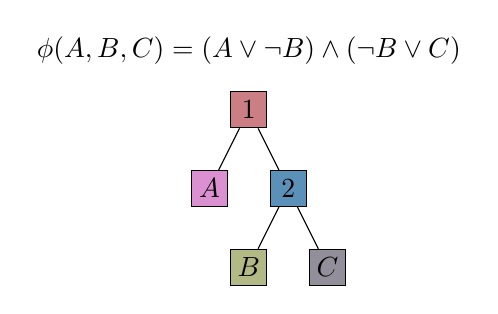
\begin{tikzpicture}
      \node at (0,0) {$\phi(A,B,C)=(A\vee\neg B)\wedge(\neg B\vee C)$};
      \newVtreeNode[fill=boxred!70]{vr}{0,-0.75}{1};
      \newVtreeNode[fill=boxblue!80]{vc}{$(vr) + (0.5,-1)$}{2};
      \newVtreeNode[fill=boxpink!50]{a}{$(vr) + (-0.5,-1)$}{$A$};
      \newVtreeNode[fill=boxgoldenrod!60]{b}{$(vc) + (-0.5,-1)$}{$B$};
      \newVtreeNode[fill=boxpurple!50]{c}{$(vc) + (0.5,-1)$}{$C$};
      \draw (vr) -- (vc) -- (b); \draw (vr) -- (a);
      \draw (vc) -- (c);
    \end{tikzpicture}
    }
  \end{vhcenterb}
\end{minipage}
\begin{minipage}[t][0.75\textheight][t]{0.45\textwidth}
  \begin{vhcenterb}
    \resizebox{0.7\textwidth}{!}{
    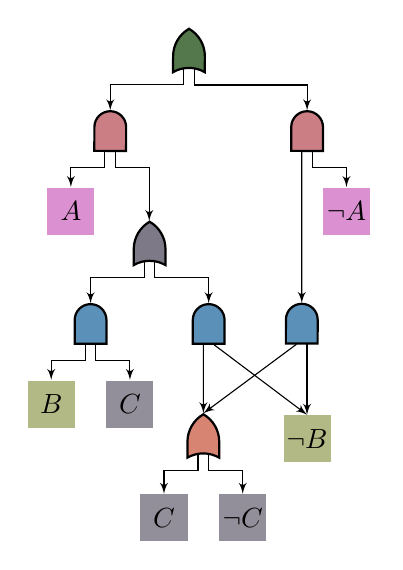
\begin{tikzpicture}
      \newOrNode[inputs=nn,fill=boxgreen]{r}{0,0};
      \newAndNode[inputs=nn,fill=boxred!70]{p1}{$(r) + (-1,-1)$};
      \newAndNode[inputs=nn,fill=boxred!70]{p2}{$(r) + (1.5,-1)$};
      \newLitNode[fill=boxpink!50]{a}{$(p1) + (-0.5,-1)$}{$A$};
      \newOrNode[inputs=nn,fill=boxpurple!60]{s1}{$(p1) + (0.5,-1.45)$};
      \newLitNode[fill=boxpink!50]{na}{$(p2) + (0.5,-1)$}{$\neg A$};
      \newAndNode[inputs=nn,fill=boxblue!80]{q1}{$(s1) + (-0.75,-1)$};
      \newAndNode[inputs=nn,fill=boxblue!80]{q2}{$(s1) + (0.75,-1)$};
      \newAndNode[inputs=nn,fill=boxblue!80]{q3}{$(p2.input 1) + (0,-2.2)$};
      \newLitNode[fill=boxgoldenrod!60]{b}{$(q1) + (-0.5,-1)$}{$B$};
      \newLitNode[fill=boxpurple!50]{c1}{$(q1) + (0.5,-1)$}{$C$};
      \newOrNode[inputs=nn,fill=boxorange!80]{z1}{$(q2.input 1) + (0,-1.2)$};
      \newLitNode[fill=boxgoldenrod!60]{nb}{$(q3.input 2) + (0,-1.2)$}{$\neg B$};
      \newLitNode[fill=boxpurple!50]{c}{$(z1) + (-0.5,-1)$}{$C$};
      \newLitNode[fill=boxpurple!50]{nc}{$(z1) + (0.5,-1)$}{$\neg C$};
      \draw[edge] (r.input 1) -- ++(0,-0.2) -| (p1);
      \draw[edge] (r.input 2) -- ++(0,-0.2) -|  (p2);
      \draw[edge] (s1.input 1) -- ++(0,-0.2) -| (q1);
      \draw[edge] (s1.input 2) -- ++(0,-0.2) -| (q2);
      \draw[edge] (p1.input 1) -- ++(0,-0.2) -| (a.north);
      \draw[edge] (p1.input 2) -- ++(0,-0.2) -| (s1);
      \draw[edge] (p2.input 1) -- (q3);
      \draw[edge] (p2.input 2) -- ++(0,-0.2) -| (na.north);
      \draw[edge] (q1.input 1) -- ++(0,-0.2) -| (b.north);
      \draw[edge] (q1.input 2) -- ++(0,-0.2) -| (c1.north);
      \draw[edge] (q2.input 1) -- (z1.east);
      \draw[edge] (q2.input 2) -- (nb.north);
      \draw[edge] (q3.input 1) -- (z1.east);
      \draw[edge] (q3.input 2) -- (nb.north);
      \draw[edge] (z1.input 1) -- ++(0,-0.2) -| (c);
      \draw[edge] (z1.input 2) -- ++(0,-0.2) -| (nc);
    \end{tikzpicture}
    }
  \end{vhcenterb}
\end{minipage}
\end{center}
}
\only<2>{
\begin{center}
\begin{minipage}[t][0.75\textheight][t]{0.45\textwidth}
  \begin{vhcenterb}
    \resizebox{!}{0.2\textheight}{
    \begin{tabular}{ccc|cc}
      \hline
      $A$ & $B$ & $C$ & $\phi(\mathbf{x})$ & $p(\mathbf{x})$\\
      \hline
      0 & 0 & 0 & 1 & 0.140\\
      1 & 0 & 0 & 1 & 0.024\\
      0 & 1 & 0 & 0 & \textcolor{gray}{0.000}\\
      1 & 1 & 0 & 0 & \textcolor{gray}{0.000}\\
      0 & 0 & 1 & 1 & 0.560\\
      1 & 0 & 1 & 1 & 0.096\\
      0 & 1 & 1 & 0 & \textcolor{gray}{0.000}\\
      1 & 1 & 1 & 1 & 0.180\\
      \hline
    \end{tabular}
    }

    \vskip 0.25cm
    \resizebox{0.8\textwidth}{!}{
    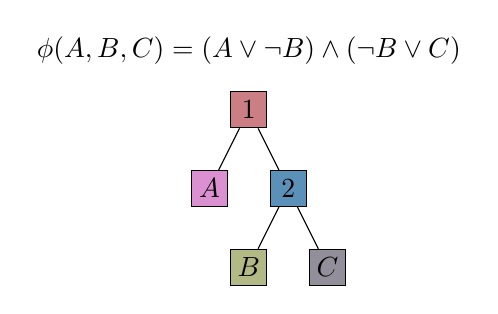
\begin{tikzpicture}
      \node at (0,0) {$\phi(A,B,C)=(A\vee\neg B)\wedge(\neg B\vee C)$};
      \newVtreeNode[fill=boxred!70]{vr}{0,-0.75}{1};
      \newVtreeNode[fill=boxblue!80]{vc}{$(vr) + (0.5,-1)$}{2};
      \newVtreeNode[fill=boxpink!50]{a}{$(vr) + (-0.5,-1)$}{$A$};
      \newVtreeNode[fill=boxgoldenrod!60]{b}{$(vc) + (-0.5,-1)$}{$B$};
      \newVtreeNode[fill=boxpurple!50]{c}{$(vc) + (0.5,-1)$}{$C$};
      \draw (vr) -- (vc) -- (b); \draw (vr) -- (a);
      \draw (vc) -- (c);
    \end{tikzpicture}
    }
  \end{vhcenterb}
\end{minipage}
\begin{minipage}[t][0.75\textheight][t]{0.45\textwidth}
  \begin{vhcenterb}
    \resizebox{0.7\textwidth}{!}{
    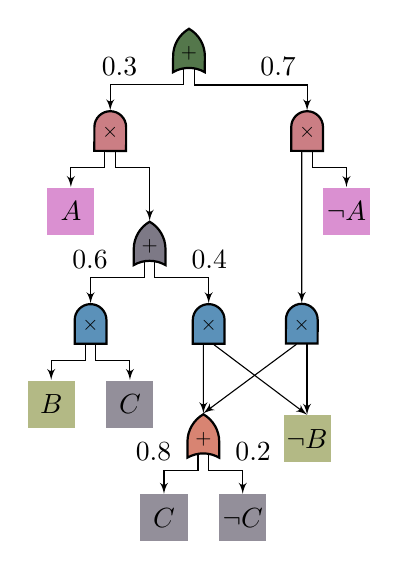
\begin{tikzpicture}
      \newNamedOrNode[inputs=nn,fill=boxgreen]{r}{0,0}{$+$};
      \newNamedAndNode[inputs=nn,fill=boxred!70]{p1}{$(r) + (-1,-1)$}{$\times$};
      \newNamedAndNode[inputs=nn,fill=boxred!70]{p2}{$(r) + (1.5,-1)$}{$\times$};
      \newLitNode[fill=boxpink!50]{a}{$(p1) + (-0.5,-1)$}{$A$};
      \newNamedOrNode[inputs=nn,fill=boxpurple!60]{s1}{$(p1) + (0.5,-1.45)$}{$+$};
      \newLitNode[fill=boxpink!50]{na}{$(p2) + (0.5,-1)$}{$\neg A$};
      \newNamedAndNode[inputs=nn,fill=boxblue!80]{q1}{$(s1) + (-0.75,-1)$}{$\times$};
      \newNamedAndNode[inputs=nn,fill=boxblue!80]{q2}{$(s1) + (0.75,-1)$}{$\times$};
      \newNamedAndNode[inputs=nn,fill=boxblue!80]{q3}{$(p2.input 1) + (0,-2.2)$}{$\times$};
      \newLitNode[fill=boxgoldenrod!60]{b}{$(q1) + (-0.5,-1)$}{$B$};
      \newLitNode[fill=boxpurple!50]{c1}{$(q1) + (0.5,-1)$}{$C$};
      \newNamedOrNode[inputs=nn,fill=boxorange!80]{z1}{$(q2.input 1) + (0,-1.2)$}{$+$};
      \newLitNode[fill=boxgoldenrod!60]{nb}{$(q3.input 2) + (0,-1.2)$}{$\neg B$};
      \newLitNode[fill=boxpurple!50]{c}{$(z1) + (-0.5,-1)$}{$C$};
      \newLitNode[fill=boxpurple!50]{nc}{$(z1) + (0.5,-1)$}{$\neg C$};
      \draw[edge] (r.input 1) -- ++(0,-0.2) -| node[near start,above left] {$0.3$} (p1);
      \draw[edge] (r.input 2) -- ++(0,-0.2) -| node[near start,above right] {$0.7$} (p2);
      \draw[edge] (s1.input 1) -- ++(0,-0.2) -| node[near start,above left] {$0.6$} (q1);
      \draw[edge] (s1.input 2) -- ++(0,-0.2) -| node[near start,above right] {$0.4$} (q2);
      \draw[edge] (p1.input 1) -- ++(0,-0.2) -| (a.north);
      \draw[edge] (p1.input 2) -- ++(0,-0.2) -| (s1.east);
      \draw[edge] (p2.input 1) -- (q3);
      \draw[edge] (p2.input 2) -- ++(0,-0.2) -| (na.north);
      \draw[edge] (q1.input 1) -- ++(0,-0.2) -| (b.north);
      \draw[edge] (q1.input 2) -- ++(0,-0.2) -| (c1.north);
      \draw[edge] (q2.input 1) -- (z1.east);
      \draw[edge] (q2.input 2) -- (nb.north);
      \draw[edge] (q3.input 1) -- (z1.east);
      \draw[edge] (q3.input 2) -- (nb.north);
      \draw[edge] (z1.input 1) -- ++(0,-0.2) -| node[near start,above left] {$0.8$} (c);
      \draw[edge] (z1.input 2) -- ++(0,-0.2) -| node[near start,above right] {$0.2$} (nc);
    \end{tikzpicture}
    }
  \end{vhcenterb}
\end{minipage}
\end{center}
}

\textcolor{dark gray}{\scriptsize\citep{kisa14}}

\end{frame}

%%%%%%%%%%%%%%%%%%%%%%%%%%%%%%%%%%%%%%%%%%%%%%%%%%%%%%%%%%%%%%%%%%%%%%%%%%%%%%%%%%%%%%%%%%%%%%%%%%%

\setbeamercolor{frametitle}{bg=palette-purple,fg=white}
\begin{frame}[fragile]{\textbf{Circuits in Visual Query Answering}}

\begin{center}
  \includegraphics[height=0.7\textheight]{figures/slash_vqa}
\end{center}

\textcolor{dark gray}{\scriptsize\citep{skryagin23}}

\end{frame}

%%%%%%%%%%%%%%%%%%%%%%%%%%%%%%%%%%%%%%%%%%%%%%%%%%%%%%%%%%%%%%%%%%%%%%%%%%%%%%%%%%%%%%%%%%%%%%%%%%%

\setbeamercolor{frametitle}{bg=palette-purple,fg=white}
\begin{frame}[fragile]{\textbf{Circuits in Natural Language Processing}}

\begin{center}
  \includegraphics[height=0.7\textheight]{figures/gelato.pdf}
\end{center}

\textcolor{dark gray}{\scriptsize\citep{zhang23}}

\end{frame}

%%%%%%%%%%%%%%%%%%%%%%%%%%%%%%%%%%%%%%%%%%%%%%%%%%%%%%%%%%%%%%%%%%%%%%%%%%%%%%%%%%%%%%%%%%%%%%%%%%%

\setbeamercolor{frametitle}{bg=palette-purple,fg=white}
\begin{frame}[fragile]{\textbf{Circuits in Neural Networks}}

\vspace{0.25cm}

\begin{center}
  \includegraphics[width=.27\columnwidth,page=2,trim=15 200 360 5,clip]{figures/spl-circ}\hfill
  \includegraphics[width=.27\columnwidth,page=3,trim=15 200 380 5,clip]{figures/spl-circ}\hfill
  \includegraphics[width=.4\columnwidth,page=1,trim=95 160 120 30,clip]{figures/spl-circ}\\[-5pt]

  \vspace{0.5cm}

  \begin{tabular}{cccc}
    \includegraphics[width=0.2\linewidth]{figures/spl-imgs/570_gt.png}
    & \includegraphics[width=0.2\linewidth]{figures/spl-imgs/570_base.png}
    & \includegraphics[width=0.2\linewidth]{figures/spl-imgs/570_sl.png}
    & \includegraphics[width=0.2\linewidth]{figures/spl-imgs/570_op.png}
    \\
    {\scriptsize\textsc{Ground Truth}} & {\scriptsize\textsc{FIL}} & {\scriptsize Semantic Loss} & 
    {\scriptsize Semantic Probabilistic Layer}
  \end{tabular}
\end{center}

\vfill

\textcolor{dark gray}{\scriptsize\citep{kareem22}}

\end{frame}

%%%%%%%%%%%%%%%%%%%%%%%%%%%%%%%%%%%%%%%%%%%%%%%%%%%%%%%%%%%%%%%%%%%%%%%%%%%%%%%%%%%%%%%%%%%%%%%%%%%

\setbeamercolor{frametitle}{bg=palette-purple,fg=white}
\begin{frame}[fragile]{\textbf{Circuits in Deep Probabilistic Logic Programming}}

\begin{center}
  \includegraphics[width=0.8\textwidth]{figures/deepproblog-diagram.pdf}

  \vspace{0.5cm}

  \begin{minipage}{0.5\textwidth}
    \centering
    \begin{minted}[fontsize=\scriptsize]{prolog}
    flip(coin1). flip(coin2).
    nn(side,C,[heads,tails])::side(C,heads);
                              side(C,tails).
    t(0.5)::red; t(0.5)::blue.
    heads :- flip(X), side(X,heads).
    win :- heads.
    win :- \+heads, red.
    query(win).
    \end{minted}
  \end{minipage}%
  \begin{minipage}{0.5\textwidth}
    \centering
    \includegraphics[width=0.9\textwidth]{figures/deepproblog-sdd.pdf}
  \end{minipage}
\end{center}

\vfill

\textcolor{dark gray}{\scriptsize\citep{manhaeve21}}

\end{frame}

%%%%%%%%%%%%%%%%%%%%%%%%%%%%%%%%%%%%%%%%%%%%%%%%%%%%%%%%%%%%%%%%%%%%%%%%%%%%%%%%%%%%%%%%%%%%%%%%%%%

\circuitslide{6}

%%%%%%%%%%%%%%%%%%%%%%%%%%%%%%%%%%%%%%%%%%%%%%%%%%%%%%%%%%%%%%%%%%%%%%%%%%%%%%%%%%%%%%%%%%%%%%%%%%%

\begin{frame}
    \titlepage
    \ccimg
\end{frame}

%%%%%%%%%%%%%%%%%%%%%%%%%%%%%%%%%%%%%%%%%%%%%%%%%%%%%%%%%%%%%%%%%%%%%%%%%%%%%%%%%%%%%%%%%%%%%%%%%%%

\nobibliography{refs.bib}

\end{document}
